% Options for packages loaded elsewhere
\PassOptionsToPackage{unicode}{hyperref}
\PassOptionsToPackage{hyphens}{url}
\PassOptionsToPackage{dvipsnames,svgnames*,x11names*}{xcolor}
%
\documentclass[
  12pt,
]{article}
\usepackage{amsmath,amssymb}
\usepackage{lmodern}
\usepackage{setspace}
\usepackage{ifxetex,ifluatex}
\ifnum 0\ifxetex 1\fi\ifluatex 1\fi=0 % if pdftex
  \usepackage[T1]{fontenc}
  \usepackage[utf8]{inputenc}
  \usepackage{textcomp} % provide euro and other symbols
\else % if luatex or xetex
  \usepackage{unicode-math}
  \defaultfontfeatures{Scale=MatchLowercase}
  \defaultfontfeatures[\rmfamily]{Ligatures=TeX,Scale=1}
\fi
% Use upquote if available, for straight quotes in verbatim environments
\IfFileExists{upquote.sty}{\usepackage{upquote}}{}
\IfFileExists{microtype.sty}{% use microtype if available
  \usepackage[]{microtype}
  \UseMicrotypeSet[protrusion]{basicmath} % disable protrusion for tt fonts
}{}
\makeatletter
\@ifundefined{KOMAClassName}{% if non-KOMA class
  \IfFileExists{parskip.sty}{%
    \usepackage{parskip}
  }{% else
    \setlength{\parindent}{0pt}
    \setlength{\parskip}{6pt plus 2pt minus 1pt}}
}{% if KOMA class
  \KOMAoptions{parskip=half}}
\makeatother
\usepackage{xcolor}
\IfFileExists{xurl.sty}{\usepackage{xurl}}{} % add URL line breaks if available
\IfFileExists{bookmark.sty}{\usepackage{bookmark}}{\usepackage{hyperref}}
\hypersetup{
  pdfauthor={Dmytro Perepolkin1,; Benjamin Goodrich2; Ullrika Sahlin1},
  colorlinks=true,
  linkcolor=Maroon,
  filecolor=Maroon,
  citecolor=Blue,
  urlcolor=Blue,
  pdfcreator={LaTeX via pandoc}}
\urlstyle{same} % disable monospaced font for URLs
\usepackage[margin=1in]{geometry}
\usepackage{color}
\usepackage{fancyvrb}
\newcommand{\VerbBar}{|}
\newcommand{\VERB}{\Verb[commandchars=\\\{\}]}
\DefineVerbatimEnvironment{Highlighting}{Verbatim}{commandchars=\\\{\}}
% Add ',fontsize=\small' for more characters per line
\usepackage{framed}
\definecolor{shadecolor}{RGB}{248,248,248}
\newenvironment{Shaded}{\begin{snugshade}}{\end{snugshade}}
\newcommand{\AlertTok}[1]{\textcolor[rgb]{0.94,0.16,0.16}{#1}}
\newcommand{\AnnotationTok}[1]{\textcolor[rgb]{0.56,0.35,0.01}{\textbf{\textit{#1}}}}
\newcommand{\AttributeTok}[1]{\textcolor[rgb]{0.77,0.63,0.00}{#1}}
\newcommand{\BaseNTok}[1]{\textcolor[rgb]{0.00,0.00,0.81}{#1}}
\newcommand{\BuiltInTok}[1]{#1}
\newcommand{\CharTok}[1]{\textcolor[rgb]{0.31,0.60,0.02}{#1}}
\newcommand{\CommentTok}[1]{\textcolor[rgb]{0.56,0.35,0.01}{\textit{#1}}}
\newcommand{\CommentVarTok}[1]{\textcolor[rgb]{0.56,0.35,0.01}{\textbf{\textit{#1}}}}
\newcommand{\ConstantTok}[1]{\textcolor[rgb]{0.00,0.00,0.00}{#1}}
\newcommand{\ControlFlowTok}[1]{\textcolor[rgb]{0.13,0.29,0.53}{\textbf{#1}}}
\newcommand{\DataTypeTok}[1]{\textcolor[rgb]{0.13,0.29,0.53}{#1}}
\newcommand{\DecValTok}[1]{\textcolor[rgb]{0.00,0.00,0.81}{#1}}
\newcommand{\DocumentationTok}[1]{\textcolor[rgb]{0.56,0.35,0.01}{\textbf{\textit{#1}}}}
\newcommand{\ErrorTok}[1]{\textcolor[rgb]{0.64,0.00,0.00}{\textbf{#1}}}
\newcommand{\ExtensionTok}[1]{#1}
\newcommand{\FloatTok}[1]{\textcolor[rgb]{0.00,0.00,0.81}{#1}}
\newcommand{\FunctionTok}[1]{\textcolor[rgb]{0.00,0.00,0.00}{#1}}
\newcommand{\ImportTok}[1]{#1}
\newcommand{\InformationTok}[1]{\textcolor[rgb]{0.56,0.35,0.01}{\textbf{\textit{#1}}}}
\newcommand{\KeywordTok}[1]{\textcolor[rgb]{0.13,0.29,0.53}{\textbf{#1}}}
\newcommand{\NormalTok}[1]{#1}
\newcommand{\OperatorTok}[1]{\textcolor[rgb]{0.81,0.36,0.00}{\textbf{#1}}}
\newcommand{\OtherTok}[1]{\textcolor[rgb]{0.56,0.35,0.01}{#1}}
\newcommand{\PreprocessorTok}[1]{\textcolor[rgb]{0.56,0.35,0.01}{\textit{#1}}}
\newcommand{\RegionMarkerTok}[1]{#1}
\newcommand{\SpecialCharTok}[1]{\textcolor[rgb]{0.00,0.00,0.00}{#1}}
\newcommand{\SpecialStringTok}[1]{\textcolor[rgb]{0.31,0.60,0.02}{#1}}
\newcommand{\StringTok}[1]{\textcolor[rgb]{0.31,0.60,0.02}{#1}}
\newcommand{\VariableTok}[1]{\textcolor[rgb]{0.00,0.00,0.00}{#1}}
\newcommand{\VerbatimStringTok}[1]{\textcolor[rgb]{0.31,0.60,0.02}{#1}}
\newcommand{\WarningTok}[1]{\textcolor[rgb]{0.56,0.35,0.01}{\textbf{\textit{#1}}}}
\usepackage{longtable,booktabs,array}
\usepackage{calc} % for calculating minipage widths
% Correct order of tables after \paragraph or \subparagraph
\usepackage{etoolbox}
\makeatletter
\patchcmd\longtable{\par}{\if@noskipsec\mbox{}\fi\par}{}{}
\makeatother
% Allow footnotes in longtable head/foot
\IfFileExists{footnotehyper.sty}{\usepackage{footnotehyper}}{\usepackage{footnote}}
\makesavenoteenv{longtable}
\usepackage{graphicx}
\makeatletter
\def\maxwidth{\ifdim\Gin@nat@width>\linewidth\linewidth\else\Gin@nat@width\fi}
\def\maxheight{\ifdim\Gin@nat@height>\textheight\textheight\else\Gin@nat@height\fi}
\makeatother
% Scale images if necessary, so that they will not overflow the page
% margins by default, and it is still possible to overwrite the defaults
% using explicit options in \includegraphics[width, height, ...]{}
\setkeys{Gin}{width=\maxwidth,height=\maxheight,keepaspectratio}
% Set default figure placement to htbp
\makeatletter
\def\fps@figure{htbp}
\makeatother
\setlength{\emergencystretch}{3em} % prevent overfull lines
\providecommand{\tightlist}{%
  \setlength{\itemsep}{0pt}\setlength{\parskip}{0pt}}
\setcounter{secnumdepth}{5}
\usepackage{dcolumn}
\usepackage{longtable}
\usepackage{natbib}
\usepackage{geometry}
\usepackage{lscape}
\usepackage{booktabs}
\usepackage{longtable}
\usepackage{array}
\usepackage{multirow}
\usepackage{wrapfig}
\usepackage{float}
\usepackage{colortbl}
\usepackage{pdflscape}
\usepackage{tabu}
\usepackage{threeparttable}
\usepackage{threeparttablex}
\usepackage[normalem]{ulem}
\usepackage{makecell}
\usepackage{xcolor}
\ifluatex
  \usepackage{selnolig}  % disable illegal ligatures
\fi
\usepackage[]{natbib}
\bibliographystyle{apalike}

\title{\vspace{1cm}The tenets of indirect inference in Bayesian models\vspace{0.5cm}}
\author{Dmytro Perepolkin\textsuperscript{1,*} \and Benjamin Goodrich\textsuperscript{2} \and Ullrika Sahlin\textsuperscript{1}}
\date{First version: 2021-06-29\\
This version: 2021-09-10}

\begin{document}
\maketitle
\begin{abstract}
\noindent\setstretch{1}
This paper extends the application of Bayesian inference to probability distributions defined in terms of its quantile function. We describe the method of \emph{indirect likelihood} to be used in the Bayesian models with sampling distributions which lack an explicit cumulative distribution function. We provide examples and demonstrate the equivalence of the ``quantile-based'' (indirect) likelihood to the conventional ``density-defined'' (direct) likelihood. We consider practical aspects of the numerical inversion of quantile function by root-finding required by the indirect likelihood method. In particular, we consider a problem of ensuring the validity of an arbitrary quantile function with the help of Chebyshev polynomials and provide useful tips and implementation of these algorithms in Stan and R. We also extend the same method to propose the definition of an \emph{indirect prior} and discuss the situations where it can be useful. \vspace{.8cm}
\end{abstract}

\setstretch{1.2}
\textsuperscript{1} Centre for Environmental and Climate Science, Lund University\\
\textsuperscript{2} Applied Statistics Center, Columbia University

\textsuperscript{*} Correspondence: \href{mailto:dmytro.perepolkin@cec.lu.se}{Dmytro Perepolkin \textless{}\href{mailto:dmytro.perepolkin@cec.lu.se}{\nolinkurl{dmytro.perepolkin@cec.lu.se}}\textgreater{}}

\setcounter{tocdepth}{4}
\tableofcontents
\renewcommand{\[}{\begin{equation}}
\renewcommand{\]}{\end{equation}}

\begin {quotation}
You have to start looking at the world in a new way.\\ 
-- Priya in TENET by Christopher Nolan 
\end{quotation}

\hypertarget{introduction}{%
\section{Introduction}\label{introduction}}

\hypertarget{aims-of-the-paper}{%
\subsection{Aims of the paper}\label{aims-of-the-paper}}

Quantile distributions are a special class of distributions with explicit quantile functions that are not analytically invertible \citep{gilchrist2000StatisticalModellingQuantile}. There have been a number of published articles where quantile distributions have been used in a context of the likelihood-free approximate Bayesian computation \citep{allingham2009BayesianEstimationQuantile, drovandi2011LikelihoodfreeBayesianEstimation, karabatsos2018ApproximateLikelihoodPerspective, fearnhead2012ConstructingSummaryStatistics, bernton2019ApproximateBayesianComputation, mcvinish2012ImprovingABCQuantile}, but the classical Bayesian inference applications have been limited \citep{haynes2005BayesianEstimationGandk, rayner2002NumericalMaximumLikelihood}.

This article attempts to build on the ideas of \citet{rayner2002NumericalMaximumLikelihood} and \citet{nair2020BayesianInferenceQuantile} and systematically present and illustrate Bayesian inference using quantile functions. We call this method of inference ``indirect'' because it deals with \emph{intermediate cumulative probabilities} (which we call \emph{depths}\footnote{Because they indicate how ``deep'' an observation is into the distribution.}) corresponding to observations (given the parametrized model). Our aim is to show that the indirect Bayesian inference using intermediate depths, leads to the same posterior beliefs, as the conventional, density-based inference. We highlight and discuss practical challenges related to inverting the non-invertible quantile functions and propose a novel application of the proxy root-finding algorithm for validation of quantile functions.

\begin{figure}

{\centering 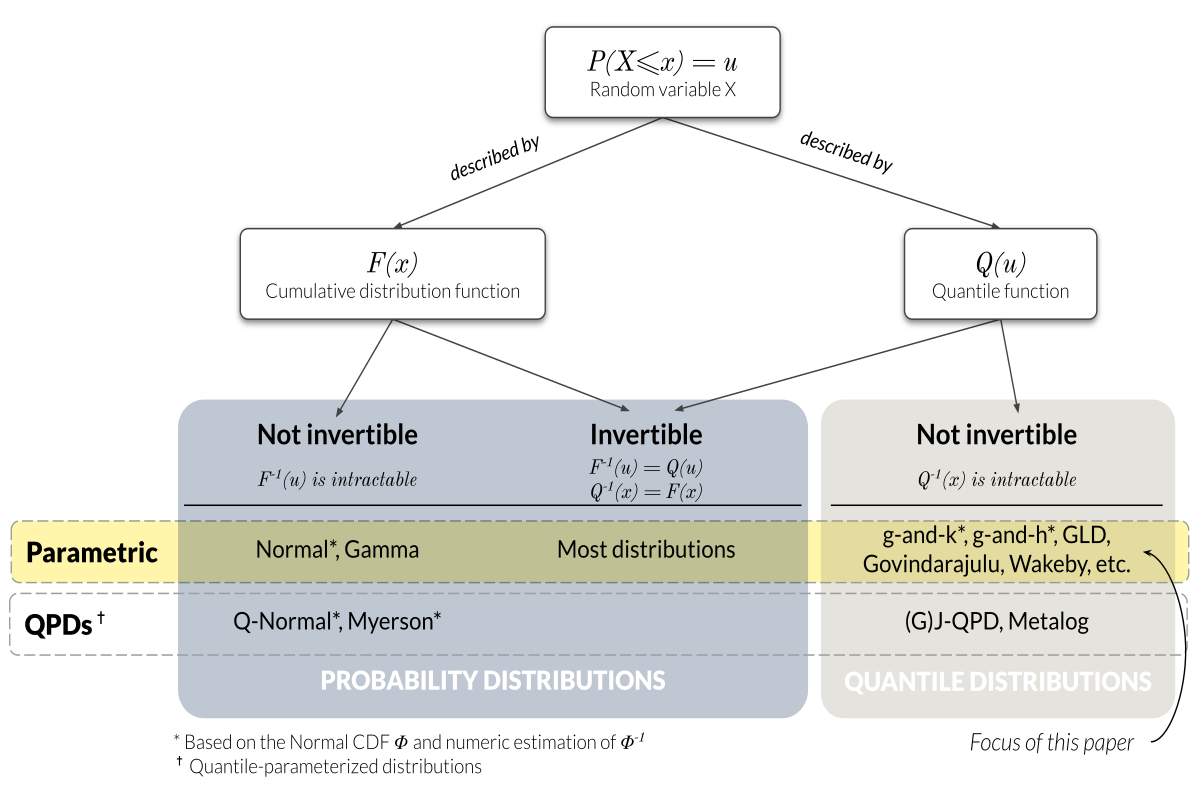
\includegraphics[width=6in]{img/QDs} 

}

\caption{Probability distributions, quantile distributions and parameterization.}\label{fig:qdist-chart}
\end{figure}

\hypertarget{paper-structure}{%
\subsection{Paper structure}\label{paper-structure}}

Section 2 revisits the functions and identities for characterizing the distribution of a continuous random variable. Then in Section 3 we introduce the terms of \emph{indirect likelihood} and \emph{indirect prior} and show that likelihood (and prior) can be expressed without the use of the probability density function (PDF). Section 4 presents an example of a Bayesian model with indirect likelihood expressed by a non-invertible quantile distribution implemented using Hamiltonian Monte Carlo in Stan \citep{standevelopmentteam2021RStanInterfaceStan}.

Section 5 discusses the computational aspects of estimating the intermediate depths in indirect likelihood expressed by a quantile distribution. We discuss root-finding algorithms and provide an example model with the indirect generalized \emph{g-and-h} \citep{haynes1997RobustnessRankingSelection} likelihood. We used the Robust Adaptive Metropolis MCMC algorithm by \citet{vihola2012RobustAdaptiveMetropolis} interfaced by the \texttt{fmcmc} package \citep{vegayon2019FmcmcFriendlyMCMC} and a built-in bracketing root-finding algorithm for inverting a quantile function in R\citep{rcoreteam2021LanguageEnvironmentStatistical}.

Section 6 discusses a problem of ensuring that the particular combination of parameters produces a valid quantile function. We propose a proxy-root-finding algorithm based on Chebyshev polynomials and discuss challenges and computational cost associated with finding the roots of a QDF. We illustrate the use of Chebyshev polynomials for proxy root-finding by approximating the quantile density function of the \emph{g-and-k} distribution and provide custom functions in R implementing the two methods of approximation proposed by \citet{boyd2013FindingZerosUnivariate}.

We conclude the paper by discussion and summary of the results in Section 7. The definitions of the distributions used in this paper are provided in Appendix A.

\hypertarget{distribution-specification}{%
\section{Distribution specification}\label{distribution-specification}}

In this section we briefly review the different ways of specifying a probability distribution to set the scene for the discussion of direct and indirect Bayesian inference. We review the use of the inverse cumulative distribution function (quantile function) to describe statistical distributions and discuss several examples of distributions defined by the quantile function (``quantile distributions'') found in the scientific literature (Figure \ref{fig:qdist-chart}).

\hypertarget{essential-functions}{%
\subsection{Essential functions}\label{essential-functions}}

Let \(X\) be a continuous random variable. It can be expressed via the distribution function, also known as the \emph{cumulative distribution function} (CDF):

\[
F_X(x | \theta)=Pr(X \leq x | \theta), \quad \theta \in \mathcal A \subset \mathbb R
\]

Alternative way of describing the random variable \(X\) is via the \emph{quantile function} (QF).

\[
Q_X(u | \theta)=\inf\{u:F_X(x|\theta)\geq u\}, \quad 0 \leq u\leq 1
\]

If \(F_X(x)\) is continuous and non-decreasing over the support of \(X\), then \(Q_X(u|\theta)\) is simply an inverse of \(F_X(x|\theta)\). Therefore, the quantile function is often referred to as the ``inverse CDF'', i.e.~

\[
Q_X(u | \theta)=F_X^{-1}(x|\theta)
\]

Not all CDFs are analytically invertible. A distribution whose quantile function \(Q_X(u | \theta)\) is not analytically invertible is called a \emph{quantile distribution} (Figure \ref{fig:qdist-chart}).

The derivative of the CDF is the \emph{probability density function} (PDF) denoted by

\[
f_X(x | \theta)=\frac{dF_X}{dx}
\]

Similarly, the derivative of the QF is the \emph{quantile density function} (QDF) denoted by

\[
q_X(u|\theta)=\frac{dQ_X}{du}, \quad 0 \leq u \leq 1
\]

The reciprocal of the QDF \([q_X(u|\theta)]^{-1}=f(Q_X(u|\theta))\) is referred to as the \emph{density quantile function} \citep{parzen1980DataModelingUsing} or \emph{p-pdf} \citep{gilchrist2000StatisticalModellingQuantile}.

\[
f(Q(u))=\frac{dF(Q(u))}{dQ(u)} = \frac{dF(Q(u))/du}{dQ(u)/du}=\frac{dF(F^{-1}(u))/du}{q(u)}=\frac{du/du}{q(u)}=[q(u)]^{-1}
\]

\hypertarget{derivatives-of-the-inverses-and-numerical-approximation}{%
\subsection{Derivatives of the inverses and numerical approximation}\label{derivatives-of-the-inverses-and-numerical-approximation}}

Following the inverse function theorem \citep{price1984InverseFunctionTheorem}, for a function to be invertible in the neighborhood of a point it should have a continuous non-zero derivative at that point. If the function is invertible, the derivative of the inverse is reciprocal to the function's derivative. Formally, if \(dy/dx\) exists and \(dy/dx \neq 0\), then \(dx/dy\) also exists and \(dx/dy=[dy/dx]^{-1}\). Therefore, for a quantile function \(Q(u)=x\), if a QDF \(q(u)\) exists and \(q(u)\neq0\), then PDF \(f(x)\) also exists and it is equal to \(f(x)=[q(u)]^{-1}\) (Figure \ref{fig:moebius-chart}). In Section 3 of this paper, we rely on the density quantile function (DQF) \([q(u|\theta)]^{-1}\), a quantile form of the PDF, to define the likelihood in a Bayesian model based on the quantile distribution.

\begin{figure}

{\centering 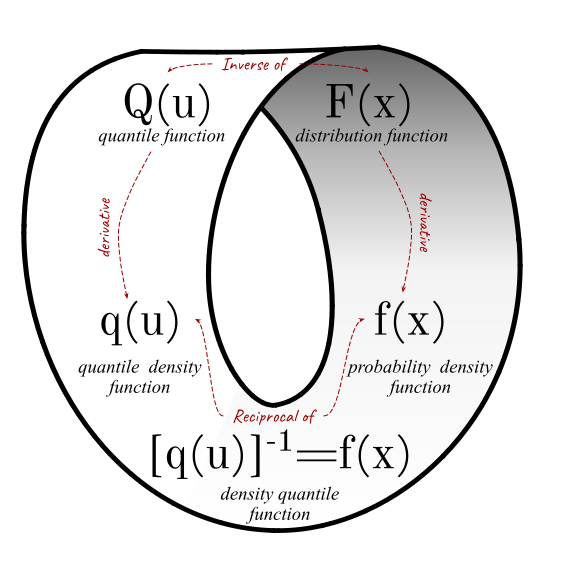
\includegraphics[width=3in]{img/moebius-loop} 

}

\caption{Moebius strip of probability functions.}\label{fig:moebius-chart}
\end{figure}

Even though quantile distributions lack the closed-form CDF \(F_X(x|\theta)=u\), in most cases, the depths \(u\) can be approximated by numerically inverting the \(Q_X(u|\theta)\). We denote the numerically inverted quantile function as \(\widehat{Q}^{-1}_X(x|\theta)\) or \(\widehat{F}_X(x|\theta)\). The inverse of a quantile function \(Q(u|\theta)\) at point \(u\), corresponding to the observation \(x\), is obtained by minimizing the difference between the actual observation \(x\) and \(Q_X(u|\theta)\) by iteratively refining the depth \(u\). The details of the numerical inversion algorithms are discussed in Section 4.

\hypertarget{quantile-distributions}{%
\subsection{Quantile distributions}\label{quantile-distributions}}

Statistical methods utilizing QF and QDF were pioneered by the seminal work of \citet{parzen1979NonparametricStatisticalData}. Today the research area of quantile distributions is an active field of interest for many scientists. The most popular quantile distributions covered in the literature are generalized \emph{g-and-h} and its sibling \emph{g-and-k} distribution \citep{haynes2005BayesianEstimationGandk, jacob2017LikelihoodCalculationGandk, prangle2017GkPackageGandk, rayner2002NumericalMaximumLikelihood}, Generalized Lambda Distribution, known as GLD \citep{aldeni2017FamiliesDistributionsArising, chalabi2012FlexibleDistributionModeling, dedduwakumara2021EfficientEstimatorParameters, fournier2007EstimatingParametersGeneralizeda, freimer1988StudyGeneralizedTukey}, Wakeby distribution \citep{rahman2015ApplicabilityWakebyDistribution} and Govindarajulu distribution \citep{nair2012GovindarajuluDistributionProperties, nair2013QuantileBasedReliabilityAnalysis}. Although in this paper we focus on the parametric quantile distributions, the quantile distributions parameterized by the quantile-probability pairs (``quantile-parametrized'' quantile distributions) are also worth a mention. The most prominent examples are the Johnson QPD (J-QPD) and its generalization \citep{hadlock2017JohnsonQuantileParameterizedDistributions, hadlock2019GeneralizedJohnsonQuantileParameterized}, as well as the metalog distribution \citep{keelin2016MetalogDistributions, keelin2011QuantileParameterizedDistributions}. These distributions play an important role in representing expert beliefs about the variables, parameters or quantities of interest, although they don't lend themselves easily as sampling distributions due to the special nature of their parameterization.

\hypertarget{bayesian-inference-with-quantile-functions}{%
\section{Bayesian inference with quantile functions}\label{bayesian-inference-with-quantile-functions}}

In this section we adopt the Bayesian updating approach proposed by \citet{rayner2002NumericalMaximumLikelihood} and \citet{nair2020BayesianInferenceQuantile} and apply it to the classical gamma-exponential model. \citet{rayner2002NumericalMaximumLikelihood} describe the three-step process of calculating the log-likelihood for a quantile distribution and use it for maximum likelihood estimation of parameters in \emph{g-and-k} and generalized \emph{g-and-h} distribution. \citet{nair2020BayesianInferenceQuantile} performed quantile function substitutions both for observables \(x_i=Q(u_i|\theta), \; u_i \in [1..N]\) and for parameters \(\theta=Q(v)\) and computed Bayes estimator under the squared error loss for Govindarajulu likelihood. In this section we try to summarize this approach and introduce the terms of \emph{direct} and \emph{indirect} likelihood based on the identities and substitutions introduced in Section 2 and show the equivalence of the two ways of expressing likelihood in Bayesian models.

\hypertarget{direct-and-indirect-likelihood}{%
\subsection{Direct and indirect likelihood}\label{direct-and-indirect-likelihood}}

Traditional Bayesian inference formula can be restated using the substitutions involving quantile functions. Assume that the prior information about the scalar parameter \(\theta\) can be summarized by the prior distribution over the parameter space, \(\Theta\). Then, given a random sample of \(\underline x=\{x_1, x_2, \dots x_n\}\), the posterior distribution of \(\theta\) can be expressed as:

\[
f(\theta|\underline{x}) \propto \mathcal{L}(\theta;\underline{x})f(\theta)
\label{eq:bayespdfeq}
\]

where \(f(\theta|\underline{x})\) is the posterior distribution of \(\theta\) after having observed the sample \(\underline{x}\), \(f(\theta)\) is the prior distribution of \(\theta\), and \(\mathcal{L}(\theta;\underline x)=\prod_{i=1}^{n}f(x_i|\theta)\) is the likelihood, which is a function of \(\theta\). We refer to this form of likelihood as ``direct'', because the observed \(\underline x\) are used as input to the likelihood function directly.

Given the random sample of \(\underline x\), we can use the quantile function to compute \(\underline{Q}=\{Q_1(u_1), Q_2(u_2), \dots Q_n(u_n)|\theta\}\), such that \(u_i=F(x_i|\theta), i=1\dots n\). The depths \(u_i\), which we denote by \(\underline u|\theta\) are degenerate random variables, because they are fully determined given the observables \(\underline{x}\) and parameter \(\theta\). Since \(Q(u_i|\theta)=x_i\) we can substitute \(\underline Q\) for \(\underline x\). Then the Bayesian inference formula \eqref{eq:bayespdfeq} becomes:

\[
f(\theta|\underline{Q}) \propto \mathcal{L}(\theta;\underline{Q})f(\theta)
\label{eq:bayesdqfeq}
\]

We refer to the likelihood \(\mathcal{L}(\theta;\underline{Q})=\prod_{i=1}^{n} f(Q(u_i|\theta))=\prod_{i=1}^n[q(u_i|\theta)]^{-1}\) as ``indirect'', because it relies on computing of intermediate depths \(u_i=F(x_i|\theta), i=1\dots n\). As we have shown, the two forms of likelihood \(\mathcal{L}(\theta;\underline{Q})\) and \(\mathcal{L}(\theta;\underline{x})\) are equal to each other. Therefore, following the likelihood principle, the posterior beliefs about \(\theta\) are equivalent.

Since the likelihood in the Equation \eqref{eq:bayesdqfeq} is expressed in terms of \(\underline {Q}=Q(\underline{u}|\theta)\), an additional transformation is required to arrive at \(\underline{u}=F(\underline{x}|\theta)\). In case a closed form of the CDF \(F(\underline x|\theta)\) is not available, the numeric approximation of \(\widehat{Q}^{-1}(\underline{x}|\theta)\) may be used. We discuss the details of the numerical approximation of the inverse quantile function in Section 5 of this paper.

To illustrate the equivalence of the two ways of specifying likelihood in Bayesian models, we use the example from \citet{klugman2004LossModelsData}\footnote{Example 16.17 on p.544} regarding the distribution of the claim amounts (referred to hereinafter, as the Claims Example).

\citet{klugman2004LossModelsData} model claim amounts using exponential distribution with the mean of \(1/\lambda\), where parameter \(\lambda\) is given the gamma prior distribution with the shape \(\alpha=4\) and the scale \(\beta=0.001\). Given three observations of the claim amounts \(\underline x=\) \{100, 950, 450\}, we sample from the posterior distribution of the parameter \(\lambda\) using the Hamiltonian Monte Carlo ``No U-Turn'' sampler implemented in Stan \citep{standevelopmentteam2021RStanInterfaceStan}. Since gamma prior is conjugate to the exponential sampling distribution \citep{pratt1995IntroductionStatisticalDecision} we can verify the distribution of the posterior draws using the analytic solution as \(f(\lambda|\underline{x})=\text{Gamma}(\lambda| \alpha+N, \beta+\sum \underline{x})\), where \(\alpha\) and \(\beta\) are the parameters of gamma distribution and \(\underline{x}=\{x_1, x_2, \dots x_N\}\) is the sample of observations of size \(N\).

Table \ref{tab:gexp-likelihood-tab} and Figure \ref{fig:gexp-likelihood-graphs} present the posterior distribution of \(\theta\) from the two gamma-exponential models: one with a direct and another one with an indirect likelihood, along with the posterior from the conjugate model. Stan programs for the corresponding examples are provided in the Supplementary Material.

\begin{table}[!h]

\caption{\label{tab:gexp-likelihood-tab}Posterior sample comparison for the models}
\centering
\begin{tabular}[t]{lrrrrr}
\toprule
model & mean & median & q5 & q95 & rhat\\
\midrule
direct likelihood & 0.0028 & 0.0027 & 0.0013 & 0.0048 & 1.000\\
indirect likelihood & 0.0028 & 0.0027 & 0.0014 & 0.0048 & 1.001\\
\bottomrule
\end{tabular}
\end{table}

\begin{figure}

{\centering 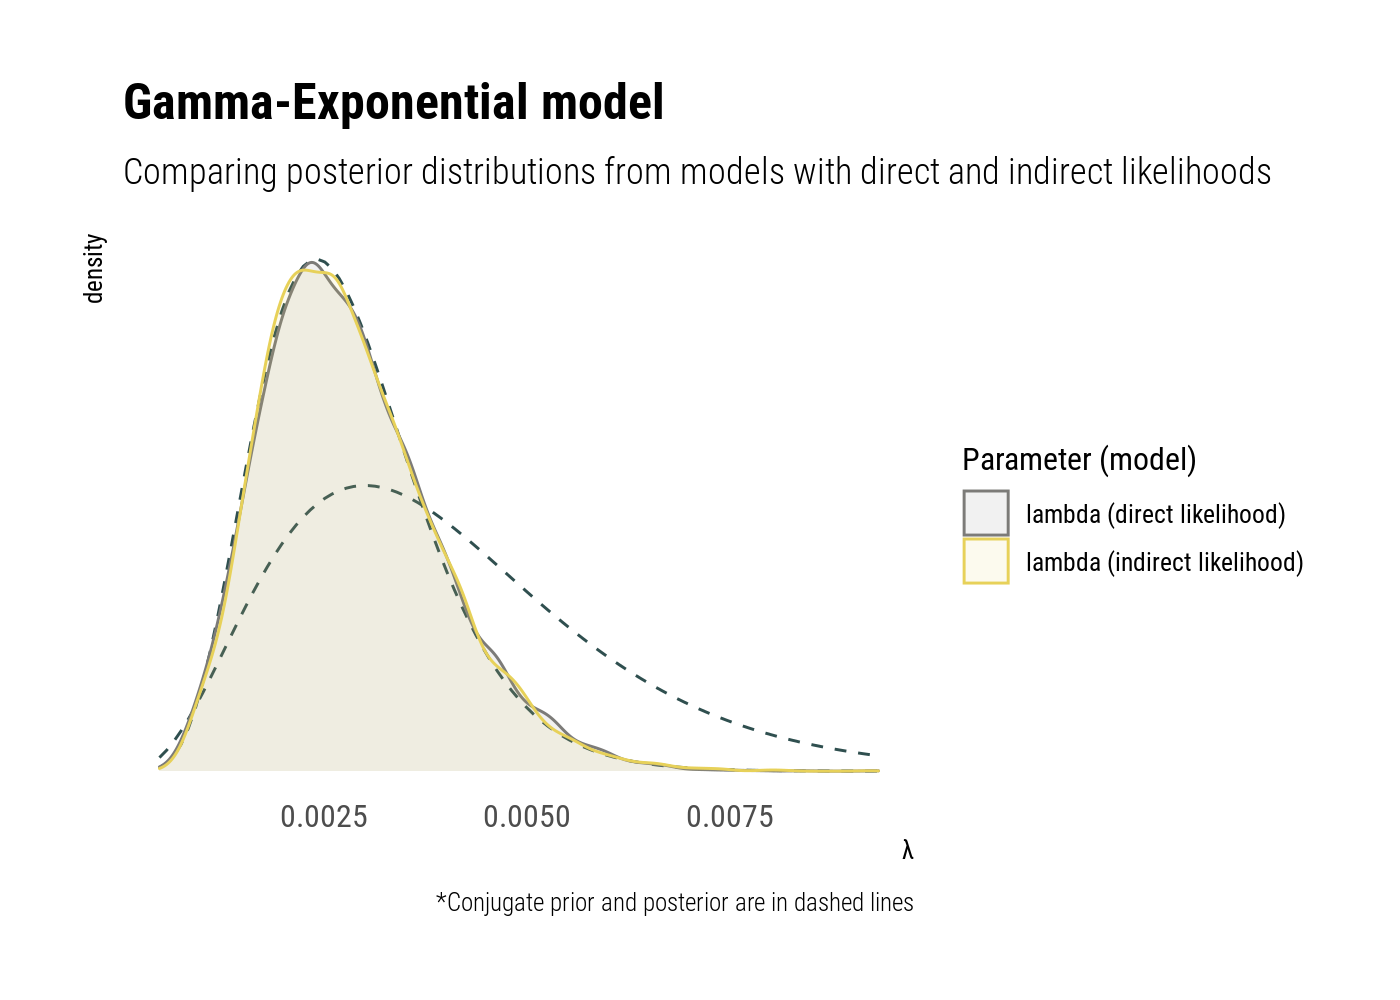
\includegraphics[width=0.8\linewidth]{ilbm_article_files/figure-latex/gexp-likelihood-graphs-1} 

}

\caption{Distribution of posterior samples from the gamma-exponential model with direct and indirect likelihood}\label{fig:gexp-likelihood-graphs}
\end{figure}

The posterior distributions of parameter \(\lambda\) from the two models are equivalent and match the analytic solution from the conjugate model within a Monte Carlo error.

\hypertarget{direct-and-indirect-prior}{%
\subsection{Direct and indirect prior}\label{direct-and-indirect-prior}}

It is possible to extend the same logic of substitution using quantile functions to define the \emph{direct} and \emph{indirect} prior. In this section we discuss the transformation of parameters required for implementing the quantile prior and show its connection to the inverse transform used for non-uniform sampling.

Bayesian inference formula can also be restated using the quantile form of the prior \citep{nair2020BayesianInferenceQuantile}. Assume that the prior distribution of \(\theta\) can be described using the invertible CDF \(F_\Theta(\theta)=v\), so that \(Q_\Theta(v)=\theta\). Substituting the quantile values \(Q_\Theta(v)\) for values of \(\theta\), prior beliefs about the parameter(s) of the distribution of \(\theta\) can be expressed \emph{indirectly} using the distribution of the quantile values corresponding to the depth \(v\), given hyperparameter(s) of the prior distribution \eqref{eq:bayesdqfdqfeq}.

\[
\begin{gathered}\;
f(Q_\Theta(v)|\underline{x}) \propto \mathcal{L}(Q_\Theta(v);\underline{x})f(Q_\Theta(v)) \\
[q_\Theta(v|\underline{x})]^{-1} \propto \mathcal{L}(Q_\Theta(v);\underline{x})[q_\Theta(v)]^{-1}
\end{gathered}
\label{eq:bayesdqfdqfeq}
\]

where \([q_\Theta(v|\underline{x})]^{-1}\) is the indirect form of the quantile posterior, \([q_\Theta(v)]^{-1}\) is the indirect form of quantile prior and \(\mathcal{L}(Q_\Theta(v);\underline{x})\) is the direct likelihood, relying on the non-linear parameter transformation \(\theta=Q_\Theta(v)\). The likelihood with such parameter transformation requires a Jacobian adjustment \citep{andrilli2010ElementaryLinearAlgebra}, which is equal to the absolute derivative of the transform, i.e.~\(J(Q_\Theta(v))=|dQ_\Theta(v)/dv|=|q_\Theta(v)|\). We refer to such formulation of the prior as the \emph{indirect prior} because it describes the prior distribution of depth \(v\) corresponding to the parameter \(\theta\) and not the distribution of the parameter \(\theta\). Therefore its density is expressed in the quantile form \(f(Q_\Theta(v))=[q_\Theta(v)]^{-1}\).

Provided that the \(Q_\Theta(v)\) is a valid (non-decreasing) quantile function, meaning that \(q_\Theta(v)\) is non-negative on \(v \in [0,1]\), the quantile density term representing the prior and the Jacobian adjustment can be dropped as they are reciprocal to each other.

\[ 
\begin{aligned}\;
&[q_\Theta(v|\underline{x})]^{-1} \propto \mathcal{L}(Q_\Theta(v);\underline{x})[q_\Theta(v)]^{-1}|q_\Theta(v)| \\
&[q_\Theta(v|\underline{x})]^{-1} \propto \mathcal{L}(Q_\Theta(v);\underline{x})
\end{aligned}
\label{eq:bayesidqfeq}
\]

where \([q_\Theta(v|\underline{x})]^{-1}\) is the quantile form of the posterior, and the quantile prior \([q_\Theta(v)]^{-1}\) is implied. The quantile function transform \(Q_\Theta(v)=\theta,v \in [0,1]\) (given the relevant hyperparameters) hints at the shape of the prior. This formulation represents the quantile function transformation of a variate with a standard uniform prior, i.e.~the unit parameter \(v\).

Indirect prior can also be used in combination with an indirect likelihood, since, as we showed previously, regardless of the form of likelihood used, the posterior beliefs about the parameter \(\theta\) (and, consequently, \(v\)) will be the same. In such a case, neither prior nor likelihood would require the existence of the closed-form PDF and, therefore, both of them can be represented by quantile distributions.

In the Claims Example the prior belief about the distribution of the exponential parameter \(\lambda\) was represented by the gamma distribution, which is not easily invertible (Figure \ref{fig:qdist-chart}). In order to illustrate the indirect specification of the prior, we pick an invertible prior as representation of the expert's beliefs about the exponential parameter \(\lambda\). The shape of the new prior \(Rayleigh(0.003)\) is comparable to the gamma prior \(Gamma(4,0.001)\) used previously (Figure \ref{fig:gamma-ray-prior-graph}).

\begin{figure}

{\centering 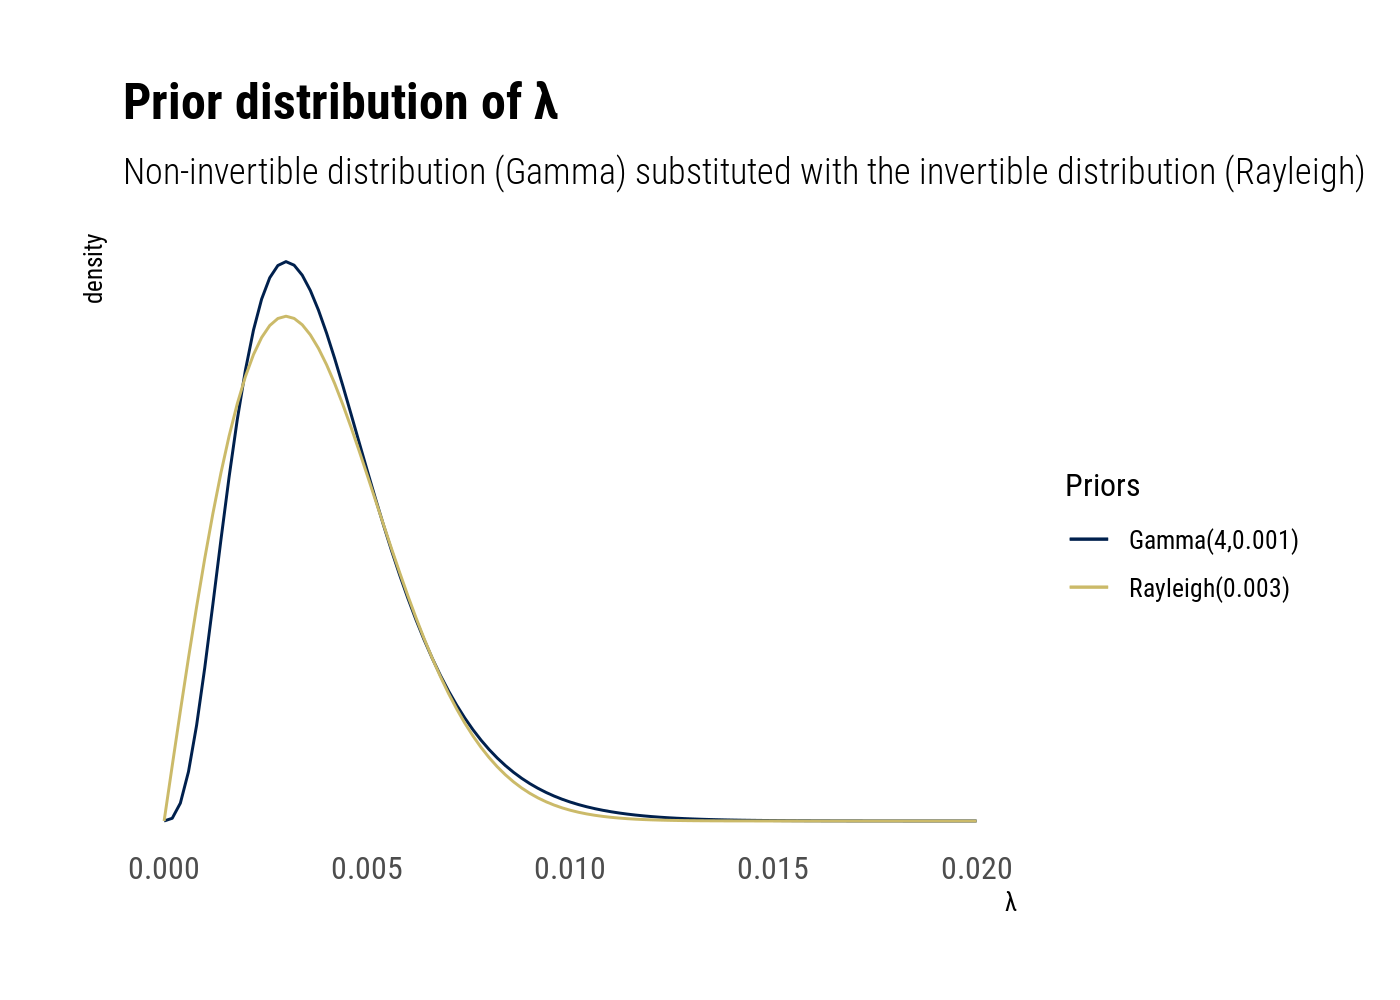
\includegraphics[width=0.8\linewidth]{ilbm_article_files/figure-latex/gamma-ray-prior-graph-1} 

}

\caption{Substitution prior for the rate parameter}\label{fig:gamma-ray-prior-graph}
\end{figure}

\begin{table}[!h]

\caption{\label{tab:rexp-prior-lik-tab}Summary of the posterior samples of the parameter lambda from the Rayleigh-Exponential model with direct and indirect prior and likelihood}
\centering
\begin{tabular}[t]{lrrrrr}
\toprule
model & mean & median & q5 & q95 & rhat\\
\midrule
direct prior, direct likelihood & 0.0027 & 0.0026 & 0.0011 & 0.0048 & 1.001\\
direct prior, indirect likelihood & 0.0027 & 0.0025 & 0.0011 & 0.0048 & 1.001\\
indirect prior, direct likelihood & 0.0027 & 0.0026 & 0.0011 & 0.0047 & 1.000\\
indirect prior, indirect likelihood & 0.0027 & 0.0026 & 0.0011 & 0.0048 & 1.001\\
\bottomrule
\end{tabular}
\end{table}

Table \ref{tab:rexp-prior-lik-tab} and Figure \ref{fig:rexp-prior-lik-graphs} compare the posterior distribution of \(\theta\) from the gamma-exponential model with direct and indirect likelihood. Stan programs for corresponding examples are provided in the Supplementary Material.

\begin{figure}

{\centering 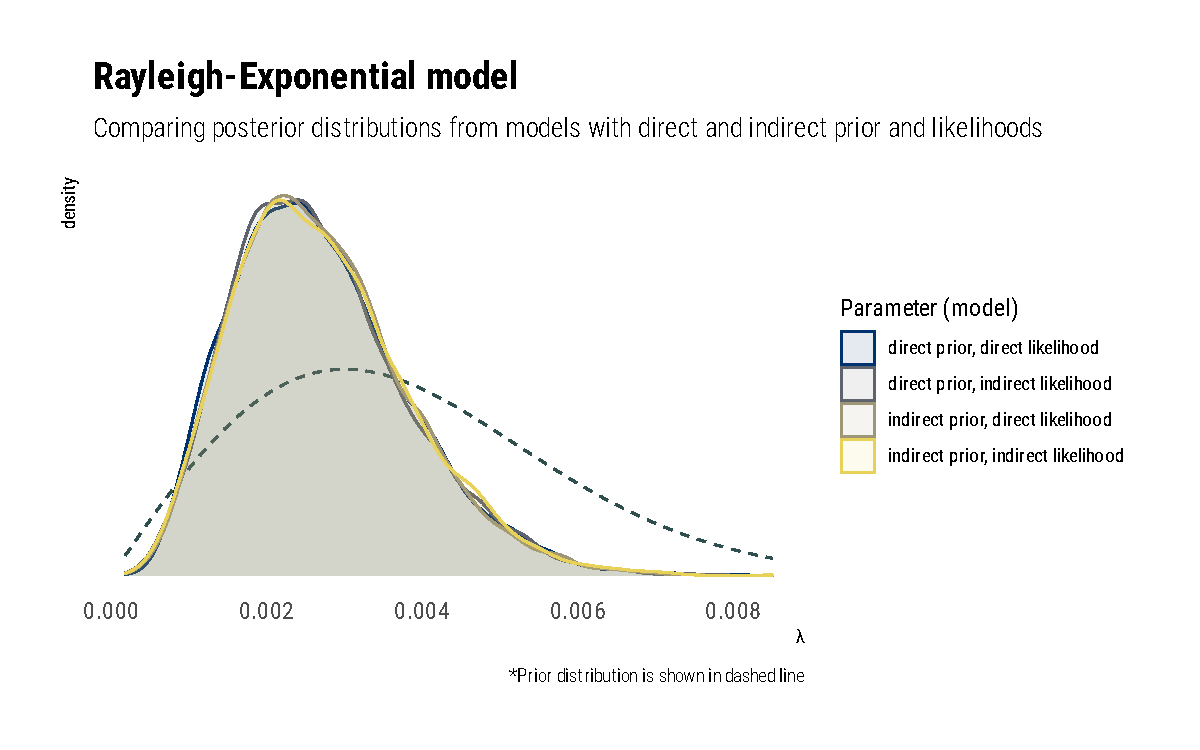
\includegraphics[width=0.8\linewidth]{ilbm_article_files/figure-latex/rexp-prior-lik-graphs-1} 

}

\caption{Distribution of the posterior samples from the Rayleigh-Exponential model with direct and indirect prior and likelihood}\label{fig:rexp-prior-lik-graphs}
\end{figure}

\hypertarget{indirect-likelihood-with-a-non-analytically-invertible-sampling-distribution}{%
\section{Indirect likelihood with a non-analytically invertible sampling distribution}\label{indirect-likelihood-with-a-non-analytically-invertible-sampling-distribution}}

The models we have used in the previous sections allowed us to choose between \emph{direct} or \emph{indirect} likelihood because the (exponential) sampling distribution was easily invertible. The main advantage of using the \emph{indirect} form of the likelihood is that it allows us to adopt the data generative model based on non-invertible (quantile) distributions. Below, we show an example of updating the parameters of a bathtub-shaped Govindarajulu distribution, which does not have a closed-form CDF or PDF.

We take the dataset provided in \citet{aarset1987HowIdentifyBathtub} on time-to-failure of 50 devices (Figure \ref{fig:bathtub-hist}). Lifetime reliability data are often modeled using specialized distributions \citep{nadarajah2009BathtubshapedFailureRate} or 2(3)-component mixtures. \citet{nair2020BayesianInferenceQuantile} used the Bayes estimator under the squared error loss function to estimate the posterior mean of the parameter \(\gamma\) in the Govindarajulu distribution \citep{nair2012GovindarajuluDistributionProperties}, given the generalized exponential prior \citep{gupta2007GeneralizedExponentialDistribution}. We extend their approach to estimate the full posterior distribution of both parameters in the Govindarajulu likelihood, implementing it in Stan \citep{standevelopmentteam2021RStanInterfaceStan}.

\begin{figure}

{\centering 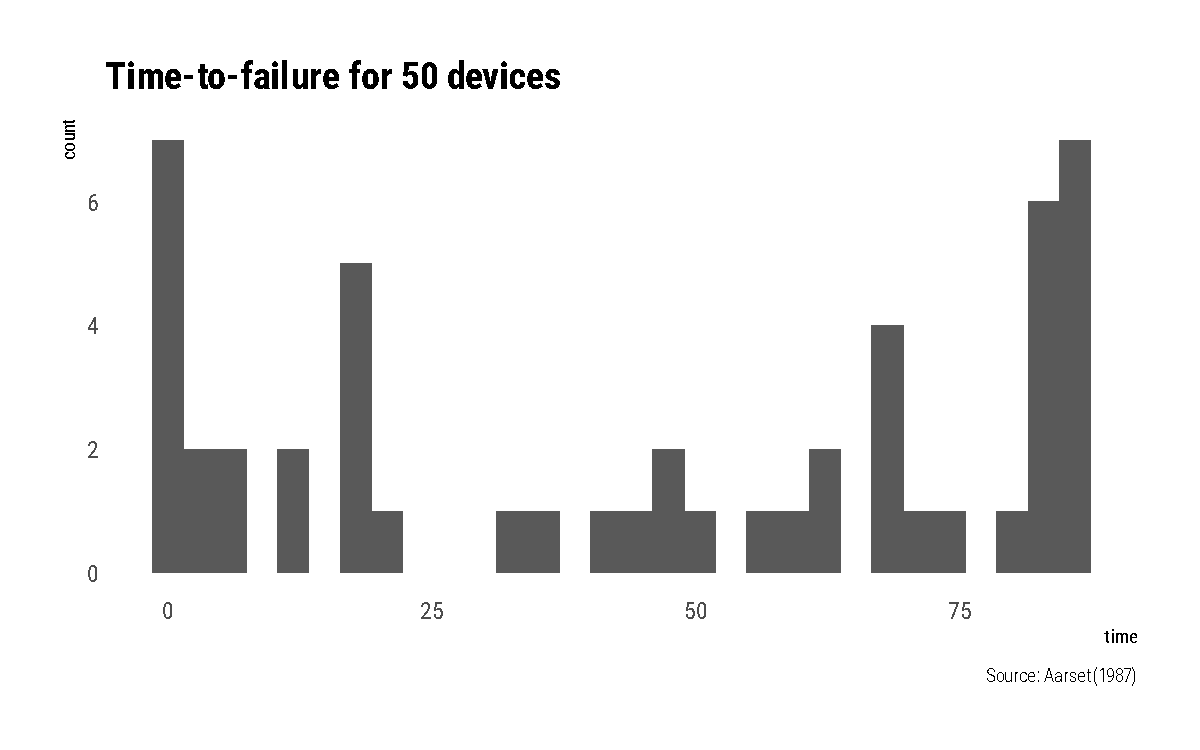
\includegraphics[width=0.8\linewidth]{ilbm_article_files/figure-latex/bathtub-hist-1} 

}

\caption{Histogram of the time to failure data}\label{fig:bathtub-hist}
\end{figure}

We adopt the generalized exponential prior for the parameter \(\gamma\) of Govindarajulu distribution with hyperparameters \(\alpha\) = 5 and \(\lambda\) = 1. The parameter \(\sigma\) of the Govindarajulu distribution can not be lower than the maximum of the observed times-to-failure. Therefore, we defined a shifted exponential prior with the rate \(\lambda\) = 1 and varying lower bound corresponding to the highest time to failure (in our example equal to 86). The Jacobian for adding a constant to the sampled parameter \(\sigma\) is equal to one, so there is no impact on the log density, as the shifting transform produces a Jacobian derivative matrix with a unit determinant.

\begin{table}[!h]

\caption{\label{tab:govi-tab}Summary of the posterior samples from the GenExp-Govindarajulu model using indirect likelihood}
\centering
\begin{tabular}[t]{lrrrrr}
\toprule
parameter & mean & median & q5 & q95 & rhat\\
\midrule
gamma & 2.0419 & 2.0128 & 1.5898 & 2.5889 & 1.001\\
sigma & 86.0216 & 86.0004 & 86.0000 & 86.1125 & 1.001\\
\bottomrule
\end{tabular}
\end{table}

\begin{figure}

{\centering 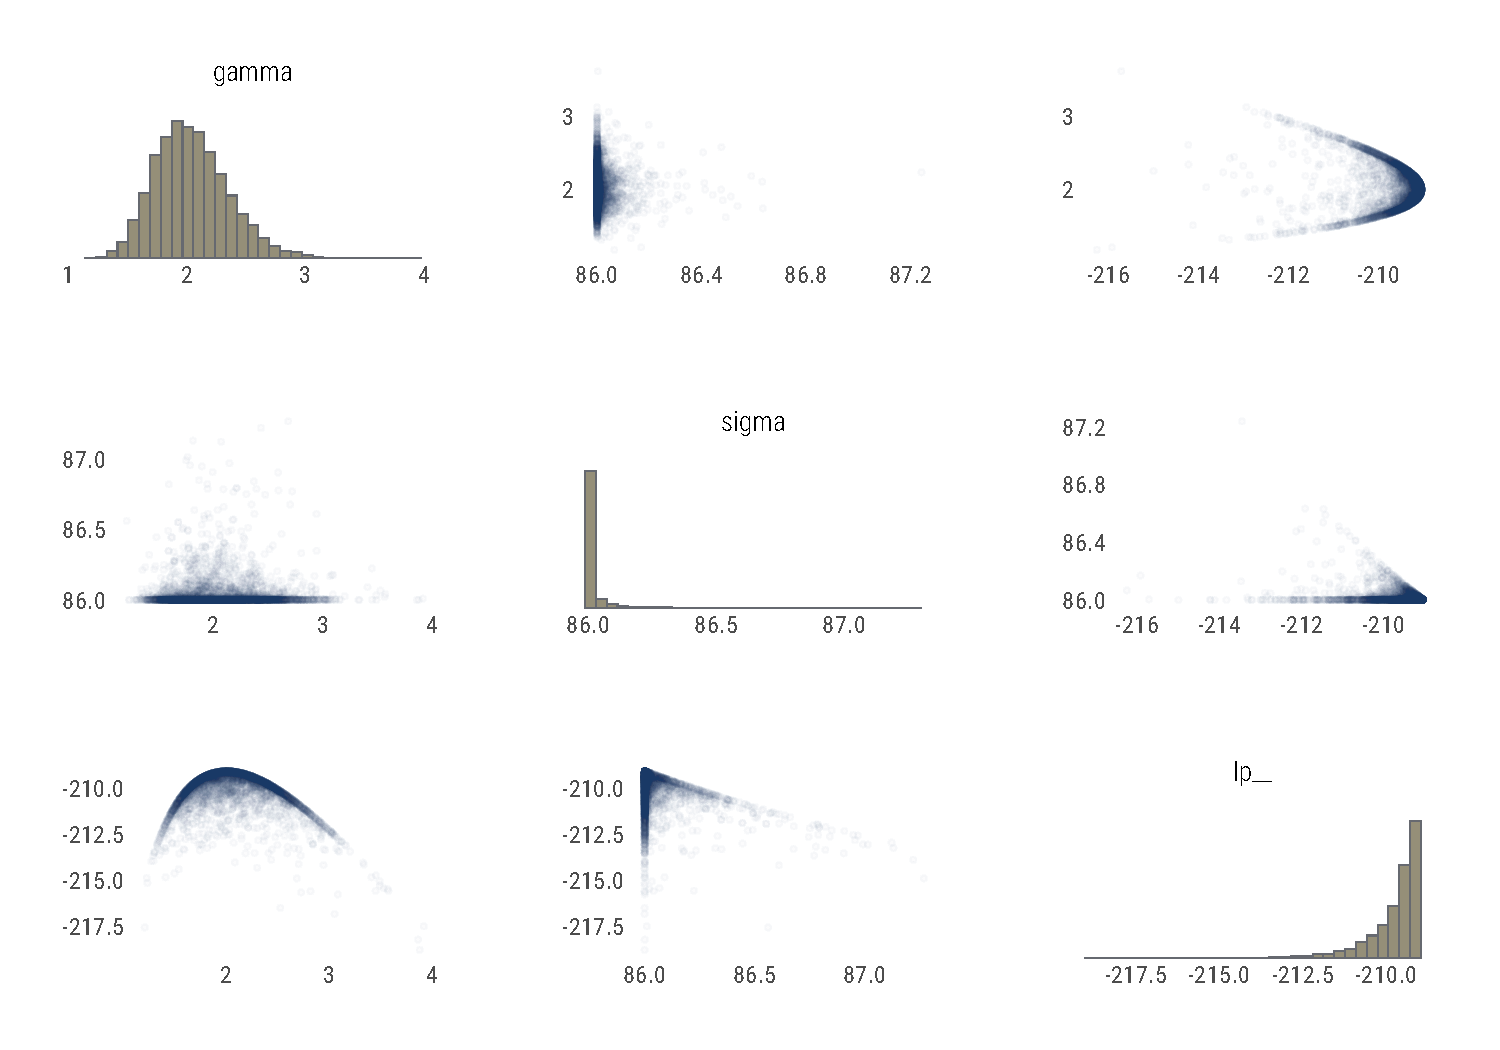
\includegraphics[width=0.8\linewidth]{ilbm_article_files/figure-latex/govi-pairs-graph-1} 

}

\caption{Posterior distribution of parameters in GenExp-Govindarajulu model}\label{fig:govi-pairs-graph}
\end{figure}

\begin{figure}

{\centering 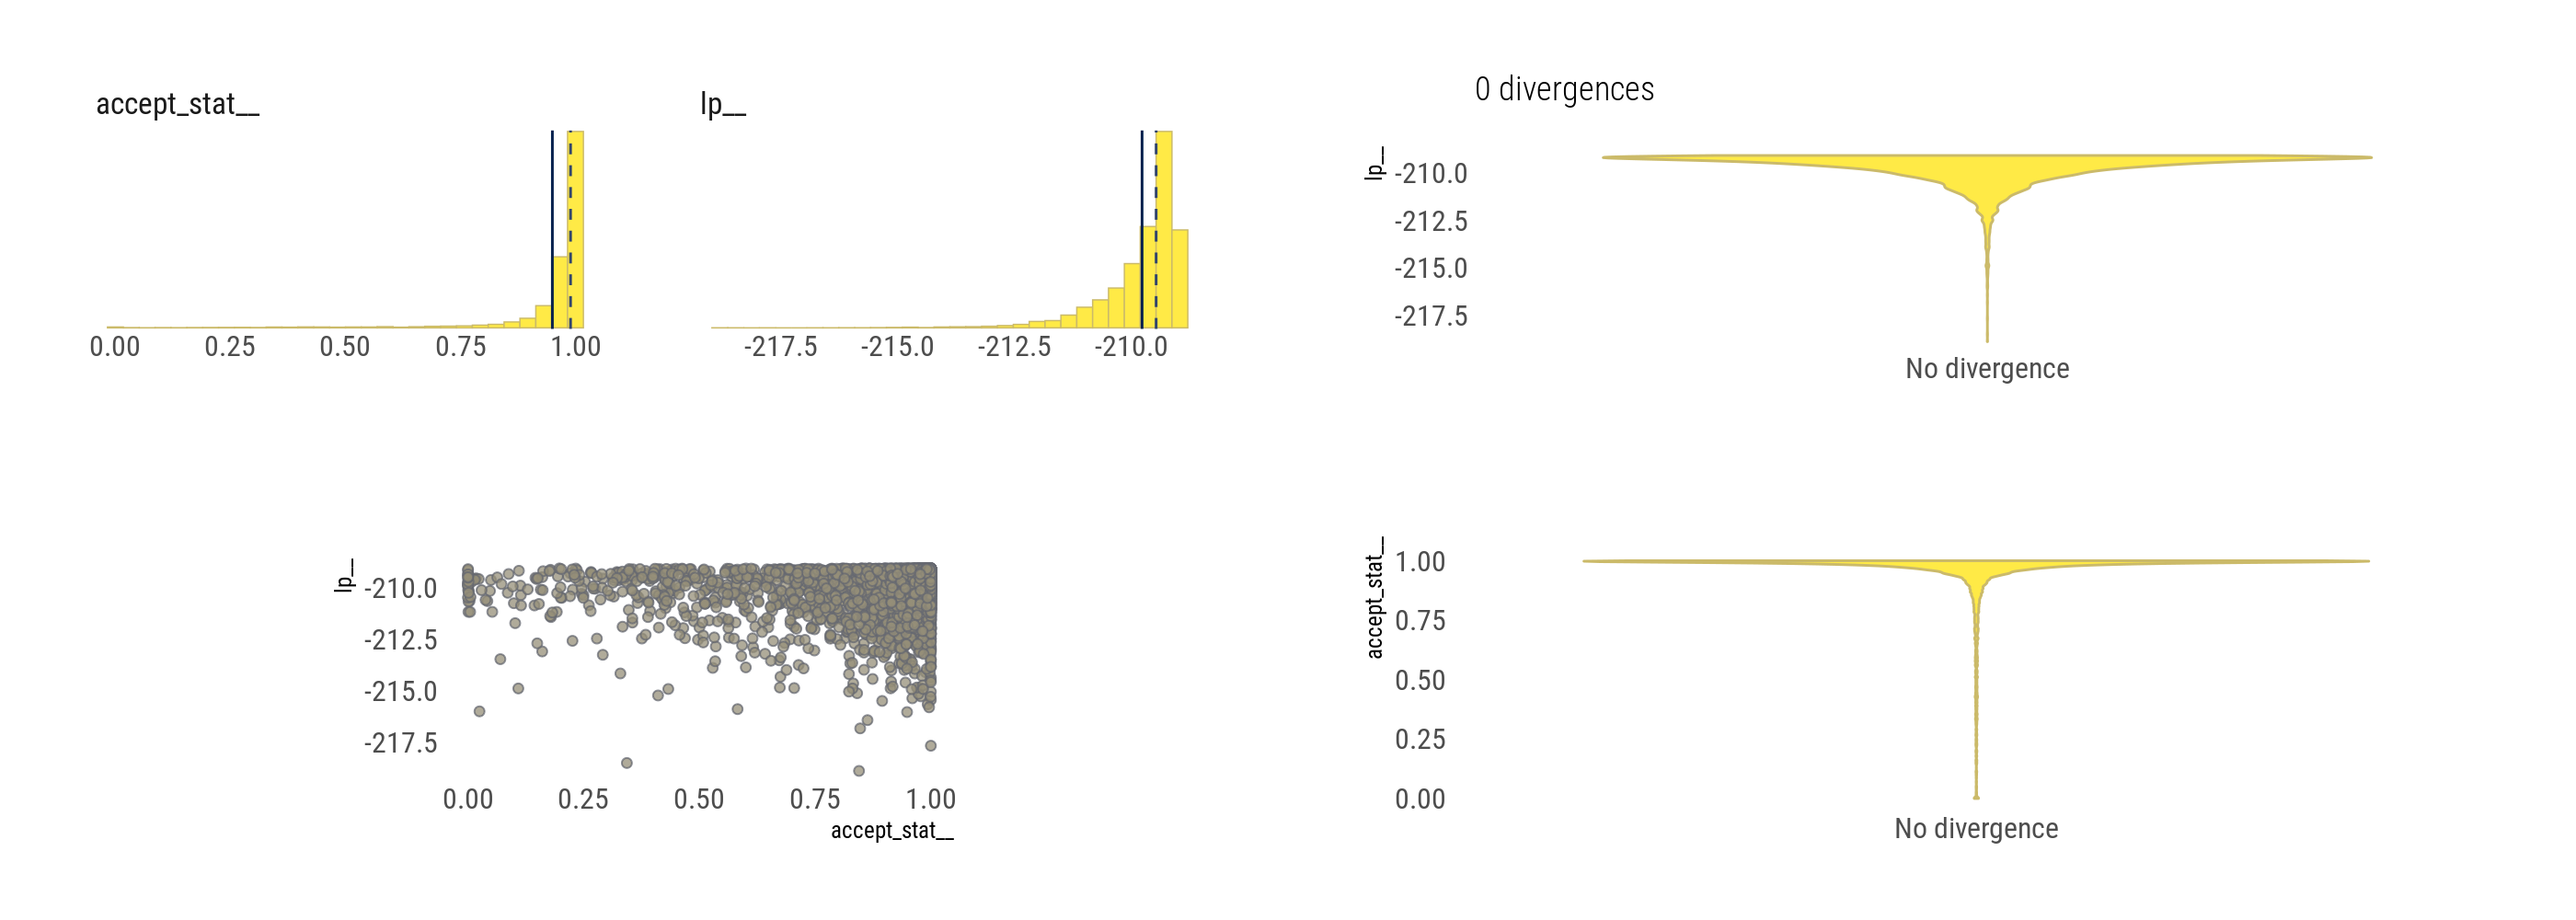
\includegraphics[width=1\linewidth]{ilbm_article_files/figure-latex/govi-nuts-graph-1} 

}

\caption{NUTS parameters for GenExp-Govindarajulu model}\label{fig:govi-nuts-graph}
\end{figure}

Table \ref{tab:govi-tab} and Figure \ref{fig:govi-pairs-graph} summarize the posterior distribution of the parameters \(\sigma\) and \(\gamma\) of Govindarajulu distribution. We used 2500 post-warmup iterations and 4 chains (see Figure \ref{fig:govi-nuts-graph} for NUTS parameter plots).

\hypertarget{numerical-inversion-of-quantile-function}{%
\section{Numerical inversion of quantile function}\label{numerical-inversion-of-quantile-function}}

The core element of the \emph{indirect} likelihood method is the use of the intermediate depths \(\underline{u}\), corresponding to the observables \(\underline{x}\) given the parameter \(\theta\). These values can either be found analytically, as \(Q^{-1}(x)=F(x)\) for probability distributions, or, numerically via root-finding algorithm, as \(\widehat{Q}^{-1}_X(x)=\widehat{F}_X(x)\) e.g.~in case of quantile distributions (Figure \ref{fig:qdist-chart}).

\hypertarget{target-function}{%
\subsection{Target function}\label{target-function}}

The problem of inverting a quantile function is tantamount to finding the root of a target function

\[
 \Omega(u;x,\theta)=[x-Q_X(u|\theta)]
\]

where \(x\) is a known observation, \(\theta\) is the parameter value, and \(u|\theta\) is the depth \(u\), such that \(\Omega(u;x,\theta)=0\). Provided that the \(Q(u|\theta)\) is a non-decreasing function and \(x\) is a fixed observable value, the target function \(\Omega(u;x,\theta)\) is non-increasing. The root-finding algorithm uses the target function to take an observable \(x\) and ``pull in'' its inverted equivalent \(Q(u|\theta)\) until the two values exactly meet by iteratively adjusting \(u|\theta\).

\hypertarget{root-finding-algorithms}{%
\subsection{Root-finding algorithms}\label{root-finding-algorithms}}

In principle, the choice of the algorithms for finding the zeros of a target function \(\Omega\) includes two broad groups of methods: \emph{bracketing} and \emph{non-bracketing} \citep{atkinson2008IntroductionNumericalAnalysis, burden2011NumericalAnalysis}.

The bracketing methods, such as bisection, secant, Lagrange polynomial and Brent method, require a pair of values around the root, i.e.~two values of \(u^+\) and \(u^-\), such that \(\Omega(u^+;x,\theta)>0\) and \(\Omega(u^-;x,\theta)<0\). In order for the algorithm to rapidly converge on a true value of probability \(u|\theta\) faster, the interval \([u^+, u^-]\) needs to be relatively narrow. One way of ensuring that the starting interval is small is via the method, which we call ``grid-matching''. Because \(Q^{-1}(x)=F(x)\) is a non-decreasing function, the interval of depths \([u^+, u^-]\) enclosing the true value \(u|\theta\) corresponding to the observable \(x\), can be found by matching the observable \(x\) to the sorted grid of \(K\) quantile values \(Q^{grd}_k=Q_X(u^{grd}_k|\theta), \quad k \in 1..K\), where \(\forall u^{grd}_k, k \in (1\dots K): 0<u^{grd}_k<1, \; u^{grd}_k<u^{grd}_{k+1}\) come from a sorted grid of depths. Once \(x\) is matched to the grid of quantiles \(Q^{grd}_k\), the quantile value immediately preceding the observable \(x\) and immediately following it, such that \(Q^{grd}_{m} \leq x \leq Q^{grd}_{m+1}\) can be determined and the corresponding depths \(u^{grd}_m\) and \(u^{grd}_{m+1}\) can be returned. The interval formed by these depths can be adopted as \([u^+, u^-]\), as it is guaranteed to contain the value of \(u\) corresponding to the root of the target function \(\Omega(u;x,\theta)\).

The non-bracketing methods, such as Newton-Rhapson, rely on a single ``initial guess'' value \(u_{(i)}\) and the gradient represented by the derivative of a target function \(\Omega^\prime(u_{(i)};x,\theta)\). Following this method the ``improved'' value \(u^*\) can found as:

\[
u^*\approx u_{(i)} -\frac{\Omega(u_{(i)};x,\theta)}{\Omega^\prime(u_{(i)};;x,\theta)}
\]

Substituting the target function \(\Omega\), the Newton-Raphson formula for finding the inverse of the quantile function becomes:

\[
u^*\approx u_{(i)}-\frac{x-Q_X(u_{(i)}|\theta)}{d[x-Q_X(u_{(i)}|\theta)]/du_{(i)}}= u_{(i)}+\frac{x-Q_X(u_{(i)}|\theta)}{q_X(u_{(i)}|\theta)}
\]

where \(u_{(i)}\) is the initial value of the probability (the ``depth'') \(u\), corresponding to the observation \(x\) given \(\theta\), \(u^*\) is the new (improved) value of \(u_{(i)}\) after an iteration and \(q_X(u_{(i)}|\theta)\) is the QDF of X, which is the first derivative of the QF \(Q_X(u_{(i)}|\theta)\) with respect to the depth \(u_{(i)}\). The procedure can be repeated by taking the approximated \(u^*\) as a new initial value \(u_{(i)}\) and recomputing the value of \(u^*\), until \(|\Omega(u_{(i)};x,\theta)|< \epsilon\), where \(\epsilon\) is some small value. For faster convergence it is desirable that the initial guess value \(u_{(i)}\) be as close to the true root as possible. The method has been used in the literature for approximating CDFs of several known quantile distributions \citetext{\citealp[see p.99 in][]{gilchrist2000StatisticalModellingQuantile}; \citealp[p.345 in][]{nair2013QuantileBasedReliabilityAnalysis}}.

There are other methods which can be adapted for finding the zeros of a function, even though they may have been developed for a different purpose. In the absence of other built-in root-finders, we used Stan's \texttt{algebra\_solver()}, intended for finding the roots of systems, to numerically determine the depths corresponding to the observable times-to-failure (see example in Section 4 above). Stan's solver is based on the Powell hybrid method, initially developed for finding the local minimum of functions. Powell's hybrid method combines the advantages of Newton's method with the steepest descent method, which guarantees stable convergence \citep{powell1970HybridMethodNonlinear}.

The rest of the section illustrates how to use the bracketing root-finding algorithm implemented in R for inverting the quantile function of the generalized \emph{g-and-h} distribution \citep{rayner2002NumericalMaximumLikelihood}. The \texttt{stats::uniroot()} function in R implements Brent's method, also known as the Brent-Dekkert algorithm, which combines the features of the bisection and secant methods with the inverse quadratic interpolation. Brent's algorithm performance ranks it only slightly behind more recent Riddler and Zhang methods \citep{stage2013CommentsImprovementBrent, zhang2011ImprovementBrentMethod}.

\hypertarget{generalized-g-and-h-distribution-and-the-normal-qdf}{%
\subsection{Generalized g-and-h distribution and the normal QDF}\label{generalized-g-and-h-distribution-and-the-normal-qdf}}

Generalized \emph{g-and-h} distribution is defined by the quantile function:

\[
Q_{gnh}(p)=A+Bz[1+C\tanh(gz/2)]\exp(hz^2/2)
\]

where \(z=z(p)=\Phi^{-1}(p|0,1)\) is the standard normal quantile function, \(B>0\) and \(h>0\). The parameter \(g\) is responsible for skewness, i.e.~when \(g<0\) the distribution is skewed left, and when \(g>0\), it is skewed right. The parameter \(h\) is responsible for kurtosis. For all values of kurtosis greater than that of the normal distribution, i.e.~\(h\geq 0\), regardless of value of \(g\), the parameter \(C \leq 0.83\) (approximately) results in a proper distribution. In practice the parameter \(C\) is often set to 0.8 \citep{haynes2005BayesianEstimationGandk, rayner2002NumericalMaximumLikelihood}.

The challenge with \emph{g-and-h} distribution is that it is expressed in terms of \(z(p)\) and not in terms of \(p\) itself. In order to differentiate the \emph{g-and-h} QF with respect to \(p\) we can use the chain rule \(q(p)=\frac{dQ}{dp}=\frac{dQ_{gnh}(z)}{dz}\frac{dz}{dp}\). The second part of this expression is the QDF of the standard normal \(\frac{dz}{dp}=\frac{d\Phi^{-1}(p)}{dp}=q_{norm}(p)\).

Even though normal distribution does not have a closed-form QF, we can exploit the fact that Stan and R have built-in functions for calculating the \(\Phi^{-1}(p)\) and derive QDF (and DQF) of the normal distribution in terms of the normal QF:

\[\frac{d\Phi^{-1}(p)}{dp}=q_{norm}(p)=[f_{norm}(Q_{norm}(p))]^{-1}=[f(\Phi^{-1}(p))]^{-1}\]

Therefore the QDF of the generalized \emph{g-and-h} distribution

\[
q_{gnh}(p)=\left(0.5B\exp(hz^2/2)[1+C\tanh(gz/2)](1+hz^2)+ \frac{Cgz}{2\cosh^2(gz/2)}\right)q_{norm}(p)
\]
where \(z=Q_{norm}(p|0,1)\) is the QF of standard normal and \(q_{norm}(p)\) is the QDF of standard normal.

\hypertarget{root-bracketing-with-grid-matching}{%
\subsection{Root bracketing with grid-matching}\label{root-bracketing-with-grid-matching}}

The \texttt{pgnh()} function in \texttt{qpd} package \citep{perepolkin2019QpdToolsQuantileparameterized} implements \(\widehat{Q}^{-1}_{gnh}(x)\) using the grid-matching method to find a pair of values bracketing the root. We use R's built-in \texttt{findInterval()} function for locating the index \(m\) of the sorted grid of \(K\) quantile values \(Q^{grd}_k=Q(u^{grd}_k|\theta), \quad k \in 1..K\), such that \(Q^{grd}_{m} \leq x \leq Q^{grd}_{m+1}\). In order to make the search of the root for the target function more numerically stable, we perform the search on the scale of \(z\)-values, i.e.~the standard normal quantile values corresponding to the depth \(p\) \citep{rayner2002NumericalMaximumLikelihood}. Once the root is found, the value of \(z\) corresponding to the root of the target function can be converted back to the depth using the standard normal CDF \(\Phi(z)=p\).

The following R code snippet implements the \(\widehat Q^{-1}_{gnh}(x)\) inverse quantile function (approximate CDF) for \emph{g-and-h} distribution

\begin{Shaded}
\begin{Highlighting}[]
\NormalTok{pgnh }\OtherTok{\textless{}{-}} \ControlFlowTok{function}\NormalTok{(q, A,B,}\AttributeTok{C=}\FloatTok{0.8}\NormalTok{,g,h, }\AttributeTok{n\_grid=}\NormalTok{100L, }\AttributeTok{s\_grid=}\NormalTok{5L, }\AttributeTok{tol=}\FloatTok{1e{-}15}\NormalTok{, }\AttributeTok{maxiter=}\FloatTok{1e3}\NormalTok{)\{}
  \CommentTok{\# target function}
\NormalTok{  afun }\OtherTok{\textless{}{-}} \ControlFlowTok{function}\NormalTok{(z, q, A,B, C, g, h) \{q }\SpecialCharTok{{-}} \FunctionTok{qgnh}\NormalTok{(z,A,B,C,g,h, }\AttributeTok{zscale=}\ConstantTok{TRUE}\NormalTok{)\}}
  \FunctionTok{stopifnot}\NormalTok{(B}\SpecialCharTok{\textgreater{}}\DecValTok{0} \SpecialCharTok{\&\&}\NormalTok{ h}\SpecialCharTok{\textgreater{}=}\DecValTok{0}\NormalTok{)}
  \CommentTok{\# service function for producing a grid of values on [0,1]}
\NormalTok{  p\_grd }\OtherTok{\textless{}{-}} \FunctionTok{make\_pgrid}\NormalTok{(}\AttributeTok{n=}\NormalTok{n\_grid, }\AttributeTok{s=}\NormalTok{s\_grid) }
\NormalTok{  q\_grd }\OtherTok{\textless{}{-}} \FunctionTok{qgnh}\NormalTok{(p\_grd, A,B,C, g,h, }\AttributeTok{zscale=}\ConstantTok{FALSE}\NormalTok{) }
\NormalTok{  idx\_lower }\OtherTok{\textless{}{-}} \FunctionTok{findInterval}\NormalTok{(q, q\_grd, }\AttributeTok{all.inside =} \ConstantTok{TRUE}\NormalTok{)}
\NormalTok{  idx\_upper }\OtherTok{\textless{}{-}}\NormalTok{ idx\_lower}\SpecialCharTok{+}\NormalTok{1L}
\NormalTok{  int\_lower }\OtherTok{\textless{}{-}}\NormalTok{ stats}\SpecialCharTok{::}\FunctionTok{qnorm}\NormalTok{(p\_grd[idx\_lower]) }\CommentTok{\# convert to z{-}scale}
\NormalTok{  int\_upper }\OtherTok{\textless{}{-}}\NormalTok{ stats}\SpecialCharTok{::}\FunctionTok{qnorm}\NormalTok{(p\_grd[idx\_upper]) }\CommentTok{\# convert  to z{-}scale}

\NormalTok{  zs }\OtherTok{\textless{}{-}} \FunctionTok{mapply}\NormalTok{(}\ControlFlowTok{function}\NormalTok{(.q, .il, .iu) \{ }\CommentTok{\# do this for every element in q}
\NormalTok{    tmp\_zs }\OtherTok{\textless{}{-}} \ConstantTok{NULL}
\NormalTok{    tmp\_zs }\OtherTok{\textless{}{-}}\NormalTok{ stats}\SpecialCharTok{::}\FunctionTok{uniroot}\NormalTok{(afun, }\AttributeTok{q=}\NormalTok{.q, }\AttributeTok{A=}\NormalTok{A, }\AttributeTok{B=}\NormalTok{B, }\AttributeTok{C=}\NormalTok{C, }\AttributeTok{g=}\NormalTok{g, }\AttributeTok{h=}\NormalTok{h, }
                             \AttributeTok{interval=}\FunctionTok{c}\NormalTok{(.il,.iu), }\AttributeTok{extendInt=}\StringTok{"downX"}\NormalTok{, }
                             \AttributeTok{check.conv=}\ConstantTok{TRUE}\NormalTok{, }\AttributeTok{tol =}\NormalTok{ tol, }\AttributeTok{maxiter =}\NormalTok{ maxiter)}
    \ControlFlowTok{if}\NormalTok{(}\FunctionTok{is.null}\NormalTok{(tmp\_zs)) res }\OtherTok{\textless{}{-}} \ConstantTok{NA\_real\_} \ControlFlowTok{else}\NormalTok{ res }\OtherTok{\textless{}{-}}\NormalTok{ tmp\_zs}\SpecialCharTok{$}\NormalTok{root }
\NormalTok{    res }\CommentTok{\#return the value of the root}
\NormalTok{  \}, q, int\_lower, int\_upper)}

\NormalTok{  ps }\OtherTok{\textless{}{-}}\NormalTok{ stats}\SpecialCharTok{::}\FunctionTok{pnorm}\NormalTok{(zs) }\CommentTok{\# convert the z values back to probability scale}

\NormalTok{  ps[}\SpecialCharTok{!}\FunctionTok{is.finite}\NormalTok{(ps)] }\OtherTok{\textless{}{-}} \ConstantTok{NA\_real\_}
\NormalTok{  ps}
\NormalTok{\}}
\end{Highlighting}
\end{Shaded}

We take a random sample of 100 values from the \emph{g-and-h} distribution with parameters A=5, B=5, C=0.8, g=5 and h=0.25. The distribution of simulated values is shown in Figure \ref{fig:gnh-data}.

\begin{figure}

{\centering 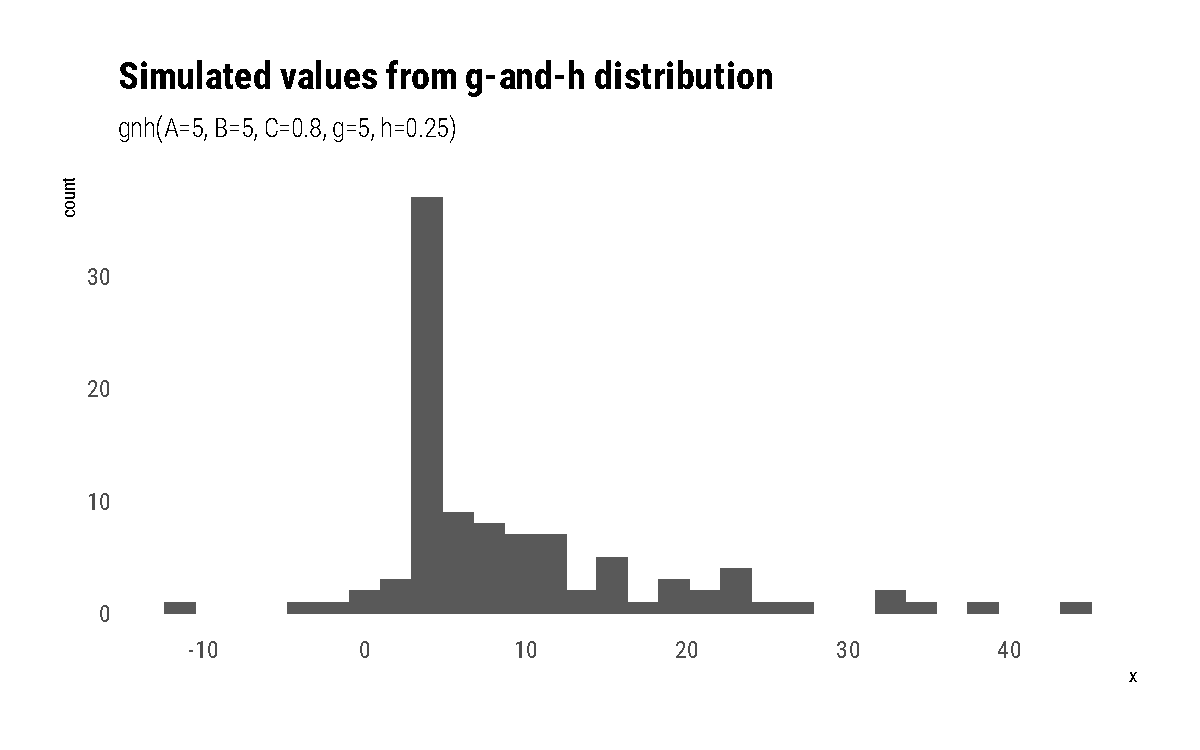
\includegraphics[width=0.8\linewidth]{ilbm_article_files/figure-latex/gnh-data-1} 

}

\caption{Simulated data from g-and-h distribution}\label{fig:gnh-data}
\end{figure}

We assumed that the parameters A and B of \emph{g-and-h} distribution are known, and defined a normal prior for parameter \(g\) as \(Normal(3,1)\) and Rayleigh prior for parameter \(h\) as \(Rayleigh(0.3)\). We performed Bayesian inference using Robust Adaptive Metropolis MCMC algorithm by \citet{vihola2012RobustAdaptiveMetropolis} interfaced by the \texttt{fmcmc} package \citep{vegayon2019FmcmcFriendlyMCMC} in R. Table \ref{tab:gnh-fit-tbl} and Figure \ref{fig:gnh-combo-graph} summarize the posterior distribution of parameters \(g\) and \(h\).

\begin{table}[!h]

\caption{\label{tab:gnh-fit-tbl}Posterior summary of parameters in g-and-h distribution}
\centering
\begin{tabular}[t]{lrrrrr}
\toprule
parameter & mean & median & q5 & q95 & rhat\\
\midrule
g & 5.0063 & 5.0136 & 4.5932 & 5.3759 & 1.003\\
h & 0.4223 & 0.4165 & 0.2912 & 0.5732 & 1.004\\
\bottomrule
\end{tabular}
\end{table}

\begin{figure}

{\centering 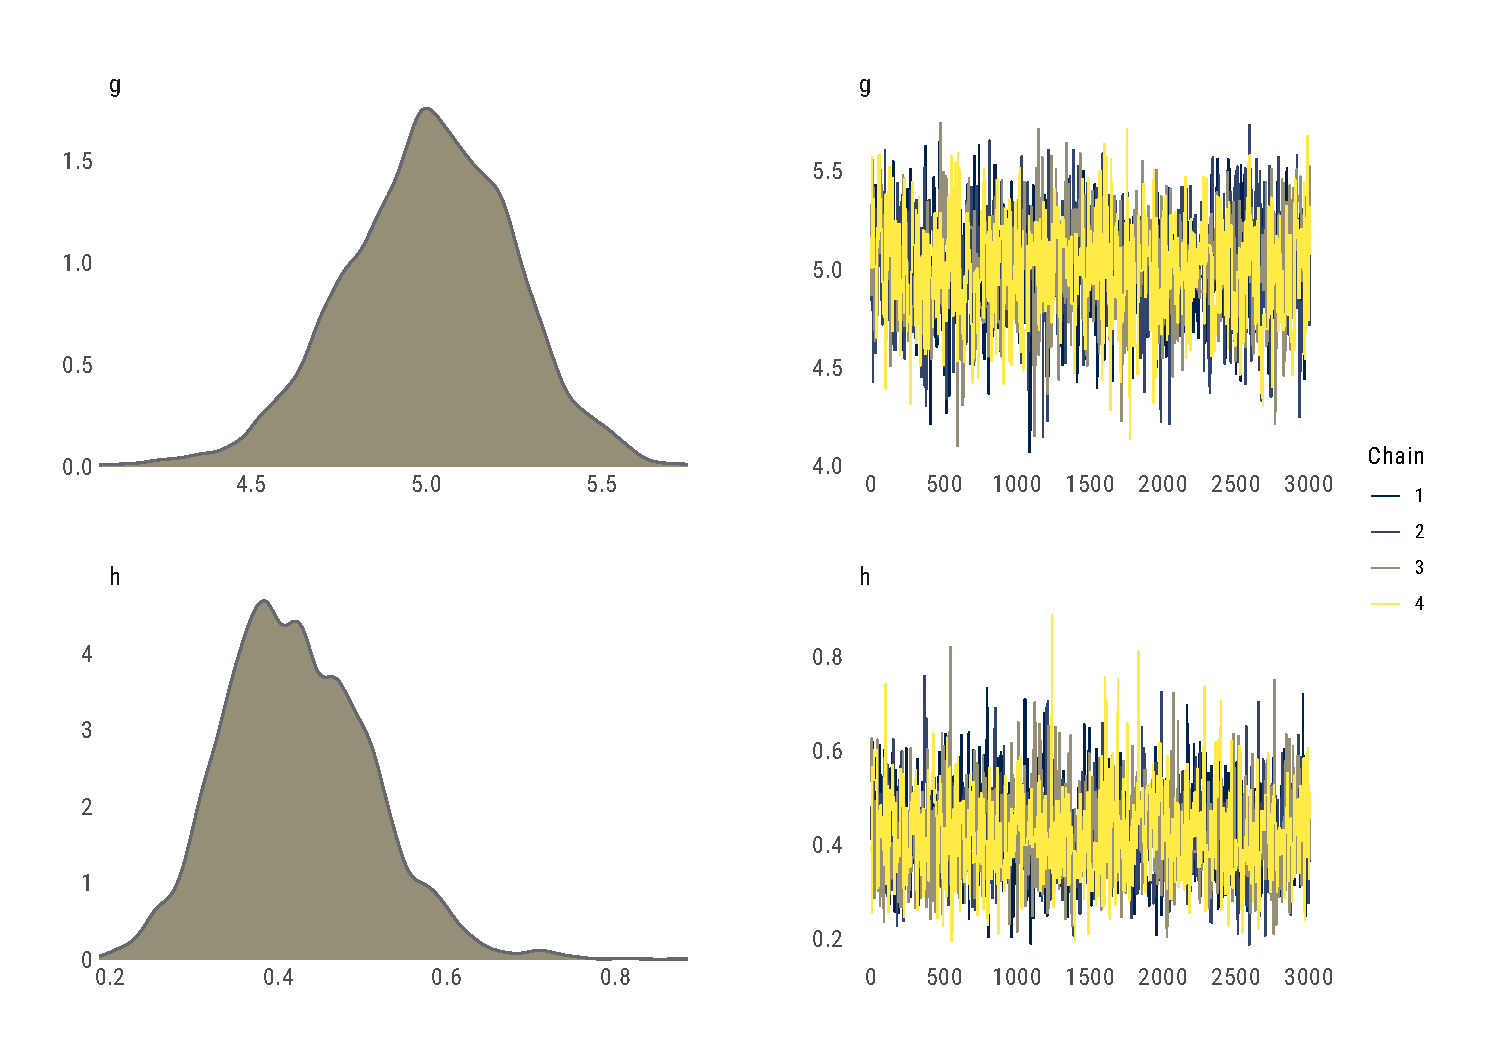
\includegraphics[width=0.8\linewidth]{ilbm_article_files/figure-latex/gnh-combo-graph-1} 

}

\caption{Posterior distribution and traceplot of parameters in g-and-h distribution}\label{fig:gnh-combo-graph}
\end{figure}

\hypertarget{validation-of-quantile-functions}{%
\section{Validation of quantile functions}\label{validation-of-quantile-functions}}

The flexibility of quantile distributions can become a curse, as certain combinations of parameters may produce an invalid quantile function. In order for the quantile function to be valid, it needs to be continuous and non-decreasing. Note that it is possible for a non-decreasing quantile function to produce a multi-modal density function and still remain valid. The violation of the QF feasibility condition manifests itself in the negative values of the QDF, measuring the rate of change in the quantile function. An invalid shape of the quantile function can cause the CDF approximation to fail both because the root-finding algorithm, such as Newton-Rhapson, can get stuck in the local minimum and because the QDF can produce an invalid gradient.

\hypertarget{parameter-conditions}{%
\subsection{Parameter conditions}\label{parameter-conditions}}

In some instances it is possible to avoid problematic cases by limiting the allowable range of parameter values. However, in highly parameterized quantile distribution, parameters may be mutually dependent, which makes it impossible to limit the problematic cases by imposing restrictions on each parameter independently. For example, Wakeby distribution has five parameter conditions, four of which are related to more than one parameter (simultaneous conditions), some of which are mutually exclusive, e.g.~``either \(\beta+\sigma>0\) or \(\beta=\gamma=\delta=0\)''. These complex conditions and bounds imposed on parameters may also be difficult to implement in MCMC samplers.

Expressing parameter conditions requires a good understanding of the distribution, and even then there might be some combinations of parameters which produce an illegal quantile function. For example, \citet{prangle2017GkPackageGandk} and \citet{rayner2002NumericalMaximumLikelihood} discuss the range of valid parameter values for the \emph{g-and-k} distribution. The parameter \(k\) should be larger than -0.5, but some values of \(-0.5<k<0\) can also lead to a quantile function being invalid. The irregularities can be difficult to spot on the quantile function graph, but the effect on the derivative functions (QDF and DQF) can be quite dramatic.

\begin{figure}

{\centering 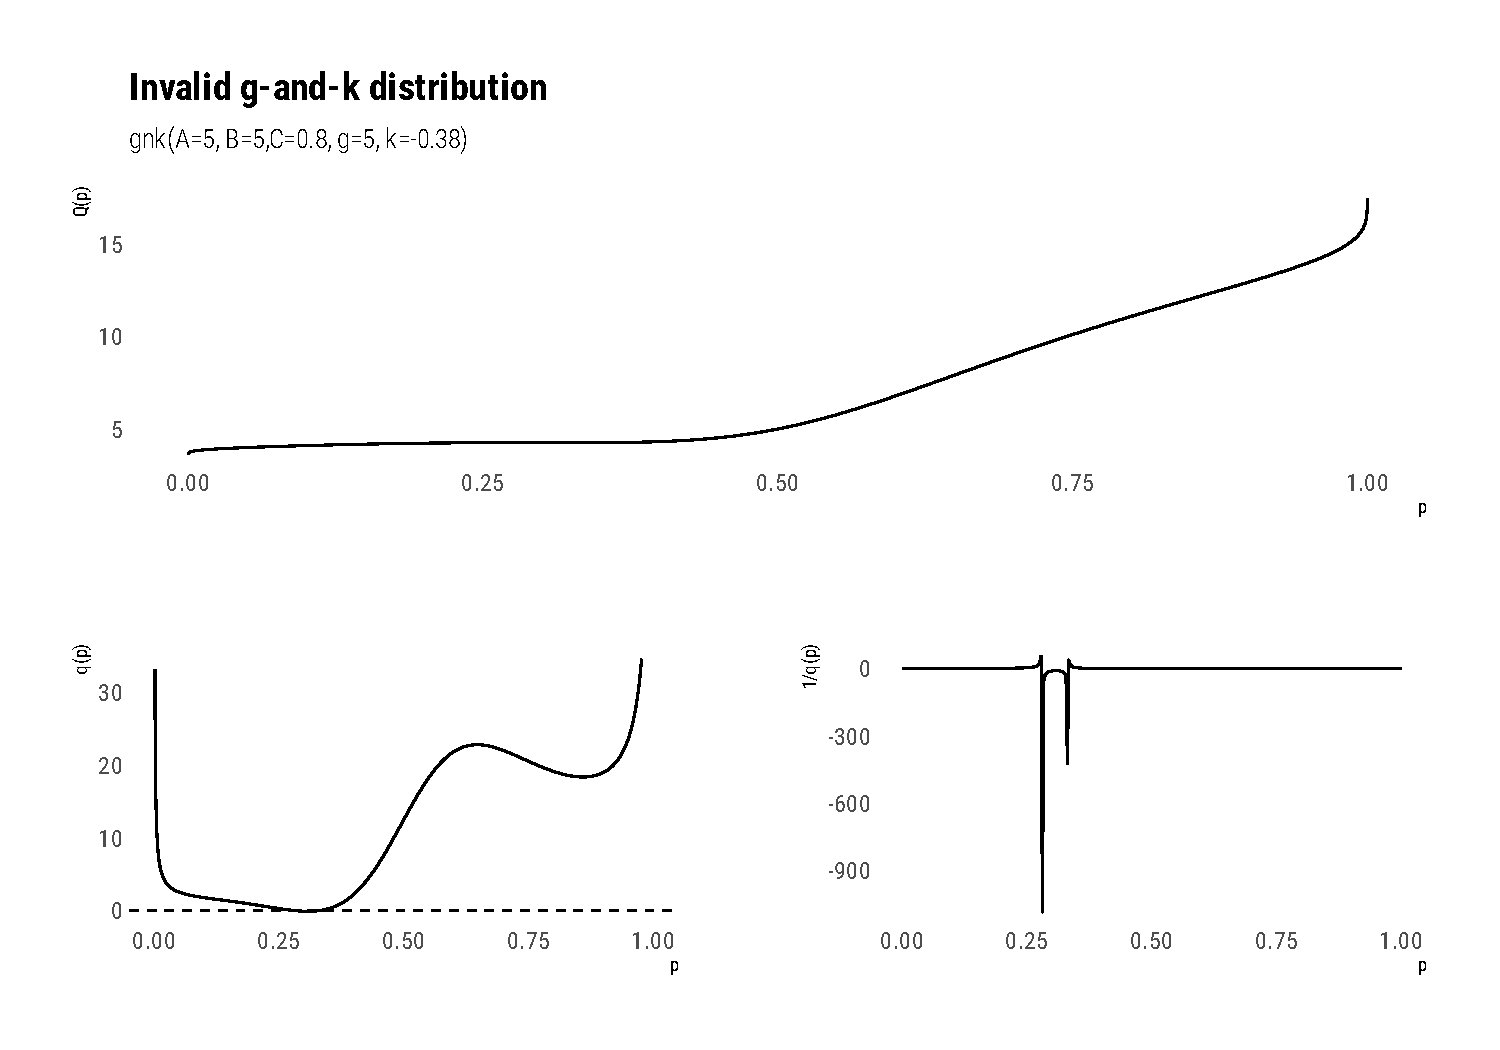
\includegraphics[width=0.8\linewidth]{ilbm_article_files/figure-latex/invalid-gnk-graph-1} 

}

\caption{Some combination of parameters of g-and-k distribution may lead to an invalid quantile function}\label{fig:invalid-gnk-graph}
\end{figure}

\hypertarget{grid-checking}{%
\subsection{Grid-checking}\label{grid-checking}}

The validity of the quantile function can also be checked by computing the QDF values corresponding to the tight grid of probabilities spread across the {[}0,1{]} range. Should any one of the QDF values be negative we can reject the quantile function with their parameters as invalid. This requires that the probability grid is tight enough to eliminate the possibility of the QDF ``dipping'' below zero between the grid values. If the cost of computing the quantile function is relatively low, and the distribution is relatively smooth (no sharp wiggles) this strategy can be reasonable. For a very tight probability grid, though, this method can become computationally expensive.

\hypertarget{global-minimum-check}{%
\subsection{Global minimum check}\label{global-minimum-check}}

An alternative approach may include finding the global minimum of the QDF and checking if it is positive. However, given the complex shape of the QDF (Figure \ref{fig:invalid-gnk-graph}), this may prove to be computationally expensive, as well.

\hypertarget{direct-root-finding}{%
\subsection{Direct root-finding}\label{direct-root-finding}}

A QDF can also be checked for roots. The values between the roots (or, if only one root is found, on one side of the root) are likely to be negative. Therefore if the roots are found this can indicate that the corresponding QF is invalid. The challenge with finding the QDF roots is that in most cases we can not use any of the bracketing methods, because the presence of roots is not known a-priori. The Newton-Rhapson method can also be problematic, due to difficulties of finding the ``good'' initial value. Also gradient-based methods, such as Newton-Rhapson, would require a derivative ``quantile convexity function'' (QCF) which may not be available, should the QDF be invalid. When validating the quantile function we are not interested in finding the roots of the QDF per se, but rather in using them as an indication that a QDF may take negative values on the range {[}0,1{]} and thus, that the corresponding QF is invalid.

\hypertarget{proxy-root-finding}{%
\subsection{Proxy root-finding}\label{proxy-root-finding}}

Finally, we can represent the QDF with a proxy function, the roots of which can be computed analytically. This method is referred to in the literature as the ``proxy root-finding'' and has been studied extensively \citep{boyd2013FindingZerosUnivariate}. Chebyshev polynomials are known for their ability to approximate functions of arbitrary complexity \citep{boyd2007NumericalExperimentsAccuracy}. In order to increase the precision of the approximation either higher degree polynomials should be used or the function range should be partitioned, keeping the degree of the polynomials applied on the subdivisions low \citep{boyd2006ComputingRealRoots}. The main computational load of the Chebyshev polynomial method is computing the eigenvalues of the Chebyshev-Frobenius companion matrix \citep{boyd2013FindingZerosUnivariate}. The logic of the method relying on a large number of partitions is that it might be computationally cheaper to find eigenvalues of many small matrices, than finding eigenvalues of a large matrix. The \texttt{qpd} package \citep{perepolkin2019QpdToolsQuantileparameterized} implements several functions for computing the coefficients, finding roots and evaluating the Chebyshev polynomial of arbitrary degree on any interval of a function. For QPD the full range of the function is \((0,1)\), but \texttt{qpd::is\_qdf\_valid()} can check a QDF function passed by the user using arbitrary number of subdivisions fitting the Chebyshev polynomial of a user-defined degree to every partition. Another strategy discussed in \citet{boyd2013FindingZerosUnivariate} is ``recursive partitioning'', where the algorithm start by fitting a single polynomial to the whole function range and comparing the goodness of fit (e.g.~the sum of squares) to some small value. If the error exceeds the threshold, the range is split in two and polynomials are fit to each subsegment, repeating the algorithm recursively.

Given the shape of the QDF function (most likely U-shaped) the largest error will be in the tails, so it might be a smart idea to make more splits toward the tails and less splits in the middle of the function range. We implemented an S-shaped subdivision scheme in \texttt{qpd::is\_qdf\_valid()} and compared its performance to the linearly partitioned quantile function. In Appendix B we compare the two schemes of proxy root-finding (degree of polynomial vs number of partitions) and discuss different approaches for dealing with false roots, which are an inevitable byproduct of polynomial approximation.

\hypertarget{discussion-and-conclusion}{%
\section{Discussion and conclusion}\label{discussion-and-conclusion}}

\hypertarget{indirect-inference}{%
\subsection{Indirect inference}\label{indirect-inference}}

Quantile distributions expand the menu of options available to the scientists and offer a wide selection of distributions to be used as likelihoods and/or priors. \citet{hadlock2017QuantileparameterizedMethodsQuantifying} summarizes the ideas from \citet{gilchrist2000StatisticalModellingQuantilea} and \citet{powley2013QuantileFunctionMethods} and provides a useful overview of properties of quantile functions. Using these properties and transformation rules, new distributions can be created on demand \citep{rodrigues2020FlexibleProcedureFormulating, midhu2014ClassDistributionsLinear, sankaran2016NewQuantileFunction, sankaran2018NewClassQuantile, yang2009QuantileBasedDistributionsModelling, smithson2017CDFquantileDistributionsModelling}.

In the past 20 years many examples using quantile distributions in approximate Bayesian computation (ABC) appeared in the literature \citetext{\citealp{allingham2009BayesianEstimationQuantile}; \citealp{drovandi2011LikelihoodfreeBayesianEstimation}; \citealp{dunson2005ApproximateBayesianInference}; \citealp{mcvinish2012ImprovingABCQuantile}; \citealp[and][]{smithson2017CDFquantileDistributionsModelling}}. ABC methods normally do not require computation of the likelihood, which in case of quantile distributions is convenient, as they lack an explicit CDF and PDF.

The first application of likelihood-based Bayesian inference for quantile distributions that we could identify was proposed by \citet{rayner2002NumericalMaximumLikelihood}. The method proposed by the authors is very similar to the \emph{indirect likelihood} method, but the authors used it for maximum likelihood estimation. Later \citet{haynes2005BayesianEstimationGandk} used this method to estimate the parameters in \emph{g-and-k} distribution using a custom MCMC algorithm. Recently, \citet{nair2020BayesianInferenceQuantile} offered the formulae for likelihood and prior expressed using the transformations involving the quantile functions, although applying it only to closed-form Bayes estimator of the posterior mean in Govindarajulu model. In this paper we summarized the ideas proposed by \citet{rayner2002NumericalMaximumLikelihood} and \citet{nair2020BayesianInferenceQuantile} and presented an \emph{indirect inference} method which makes quantile distributions usable as sampling distributions or priors. We also offered examples and implementation in STAN demonstrating the equivalence of using indirect likelihood and prior to the Bayesian inference using the traditional (density-based) likelihood and prior.

A class of quantile distributions, which we did not cover in this paper, namely, quantile-parameterized distributions \citep{keelin2011QuantileParameterizedDistributions, hadlock2017JohnsonQuantileParameterizedDistributions, keelin2016MetalogDistributions} can be especially useful as priors, given their highly interpretable parameterization. Further research is required in applying the principles of indirect likelihood to quantile-parametrized quantile distributions to make them useful as sampling distributions.

\hypertarget{practical-tips-for-implementing-quantile-distributions-in-stan-and-in-r.}{%
\subsection{Practical tips for implementing quantile distributions in Stan and in R.}\label{practical-tips-for-implementing-quantile-distributions-in-stan-and-in-r.}}

We implemented several quantile distributions in R (see \texttt{qpd} package) and in Stan (see Supplementary Materials) using certain conventions which might simplify their usage in other applications. First of all, we followed the prefix convention in R for naming probability functions ``p'' for CDF (e.g.~\texttt{pnorm()}), ``q'' for QF (e.g.~\texttt{qnorm()}), ``d'' for PDF (\texttt{dnorm()}) and ``r'' for random number generators (\texttt{rnorm}). We extended the prefix list for quantile distributions: ``f'' for QDF (e.g.~\texttt{fnorm()}), ``dq'' for DQF (e.g.~\texttt{dqnorm()}) and ``ff'' for QCF, second derivative of QF (e.g.~\texttt{ffnorm()}). Moreover, all approximate inverse QF (or CDF) functions have \emph{tolerance} and \emph{maximum number of iterations} arguments exposed (with reasonable default values), which indicate that even though the ``p''-prefixed function is available, it is based on the approximation. We used bracketing root-finding algorithm with grid-matching to provide initial values to the target function (exposing the control over the grid to the user).

In Stan, custom functions are implemented in the \texttt{functions\{\}} block. In most cases we had to implement a QF (for various transformations, including inside target function), sometimes both vectorized and scalar version, because user functions in Stan can have only one signature. We also implemented a QDF to be used, for example, in the Newton-Rhapson method, and as a service function inside the DQF. Because DQF is used in likelihood, Stan requires that the function name ends with \texttt{\_lpdf} suffix. Should the tilde sampling notation be used, the suffix can be omitted. We hope that in the future quantile density suffix \texttt{\_ldqf} will be accepted as well, but until that time we opted for double-suffixing.

As we mentioned, Stan allows only one signature for user function per name. Although it is possible to implement a vectorized log-DQF function to be used for likelihood, we opted for the scalar version (and therefore use it inside the loop over the observations). Implementing a scalar version of the log-density-quantile function is unavoidable for specification of the indirect prior, so in order to minimize the code repetition we used the scalar version for the likelihood as well. In the process of testing the Stan code, none of our custom probability functions caused problems or divergences. Challenges were more often caused by the lookup function (which performs the grid-matching) or the root-finding functions (we used built-in \texttt{algebra\_solver()}). We could not get the recently implemented \texttt{algebra\_solver\_newton()} to work inside the indirect likelihood without divergences, so we used the default Powell hybrid algorithm. When implementing custom functions that will be used outside of the \texttt{transformed\ data\{\}} block, the usage of step-like functions should be minimized, in order to avoid possible issues with divergent transitions (see Stan Functions Reference Section 3.7 for details).

We calculated the CDF-values \(\underline u\) directly in the model block inside the likelihood loop and not as \texttt{transformed\ parameters\{\}}. Below is the example of the \texttt{model\{\}} block from our GenExp-Govindarajulu model. Implementing 1D root-finding using the solver for linear algebra is a little awkward. We hope Stan will get its own (``auto-diffable'') Brent's root-finder soon.

\begin{verbatim}
model {
  vector[N] u;
  // create grid of quantile values
  vector[M] xs_grd = govindarajulu_v_qf(ys_grd, gamma, sigma);
  // look-up u corresponding to closes value from the grid
  vector[N] u_guess = vlookup(x_srt, xs_grd, ys_grd);
  // priors
  target += genexp_s_lpdf(gamma | genexp_alpha, genexp_lambda);
  target += exponential_lpdf(dsigma | exp_lambda);
  // likelihood
  for (i in 1:N){
   // numerical inversion
   u[i] = approx_govindarajulu_cdf_algebra(x_srt[i], u_guess[i], gamma, sigma, rel_tol, f_tol, max_steps);
   // likelihood statement
   target += govindarajulu_s_ldqf_lpdf(u[i] | gamma, sigma);
  }
}
\end{verbatim}

We found that when using \emph{indirect} inference (both in Stan and in R), good initial values are essential. We tried to cue initial values closer to the mode of the prior to facilitate better mixing of MCMC chains.

\hypertarget{conclusion}{%
\subsection{Conclusion}\label{conclusion}}

Embracing and expanding the use of quantile distributions in Bayesian inference can enable new solutions for old problems and enrich the toolkit available to scientists for performing hard inference tasks. We hope that the \emph{indirect} inference methods presented in this paper can contribute to expanding the body of knowledge in Bayesian statistics and fuel further research in the area of quantile distributions.

\hypertarget{miscellaneous}{%
\section*{Miscellaneous}\label{miscellaneous}}
\addcontentsline{toc}{section}{Miscellaneous}

\hypertarget{acknowledgments}{%
\subsection*{Acknowledgments}\label{acknowledgments}}
\addcontentsline{toc}{subsection}{Acknowledgments}

The authors have no conflict of interest to declare. D Perepolkin was funded by the strategic research environment Biodiversity and Ecosystem
Services in Changing Climate (BECC). U Sahlin was funded by the Swedish research council FORMAS through the project ``Scaling up
uncertain environmental evidence'' (219‐2013‐1271) and the strategic research environment Biodiversity and Ecosystem
Services in Changing Climate (BECC).

\hypertarget{data-availability-statement}{%
\subsection*{Data Availability Statement}\label{data-availability-statement}}
\addcontentsline{toc}{subsection}{Data Availability Statement}

The \texttt{qpd} R package used in this paper is available on Github at \url{https://github.com/dmi3kno/qpd}. Contact corresponding author Dmytro Perepolkin (\href{mailto:Dmytro.Perepolkin@cec.lu.se}{\nolinkurl{Dmytro.Perepolkin@cec.lu.se}}) for requests for data.

\hypertarget{supplemental-materials}{%
\subsection*{Supplemental materials}\label{supplemental-materials}}
\addcontentsline{toc}{subsection}{Supplemental materials}

Supplemental materials contain R and Stan code for all examples used in the article.

\hypertarget{orcid}{%
\subsection*{ORCID}\label{orcid}}
\addcontentsline{toc}{subsection}{ORCID}

Dmytro Perepolkin \url{https://orcid.org/0000-0001-8558-6183}\\
Ullrika Sahlin \url{http://orcid.org/0000-0002-2932-6253}

\hypertarget{appendix-a.-distributions-used-in-the-paper}{%
\section*{Appendix A. Distributions used in the paper}\label{appendix-a.-distributions-used-in-the-paper}}
\addcontentsline{toc}{section}{Appendix A. Distributions used in the paper}

\hypertarget{exponential-distribution}{%
\subsection*{Exponential distribution}\label{exponential-distribution}}
\addcontentsline{toc}{subsection}{Exponential distribution}

Exponential distribution function \(F(x)\) and the probability density function \(f(x)\) are given by

\[
\begin{gathered}
F(x)=1-e^{-\lambda x} \\ 
f(x)=\lambda e^{-\lambda x}
\end{gathered}
\]

where \(\lambda>0\) and \(x\in[0,\infty)\).

Exponential quantile function \(Q(u)\) and quantile density function \(q(u)\) are

\[
\begin{gathered}
Q(u)=-\frac{\ln(1-u)}{\lambda}\\ 
q(u)=\frac{dQ(u)}{du}=\frac{1}{\lambda(1-u)}
\end{gathered}
\]

where \(\lambda>0\) and \(u=F(x), u \in [0,1]\)

\hypertarget{rayleigh-distribution}{%
\subsection*{Rayleigh distribution}\label{rayleigh-distribution}}
\addcontentsline{toc}{subsection}{Rayleigh distribution}

Rayleigh distribution function \(F(x)\) and probability density function \(f(x)\) are:

\[ 
\begin{gathered}\;
F(x|\sigma) = 1-\exp(-x^2/(2\sigma^2)) \\ 
f(x|\sigma) = \frac{x}{\sigma^2}\exp(-x^2/(2\sigma^2))
\end{gathered}
\]

where \(\sigma>0\) is Rayleigh scale parameter.

Rayleigh quantile function \(Q(p)\) and quantile density function \(q(p)\) are:

\[
\begin{gathered}\;
Q(p|\sigma)=\sigma\sqrt{-2\ln(1-p)} \\ 
q(p|\sigma)=\frac{\sigma}{\sqrt{2}\sqrt{-\ln(1-p)}(1-p)}
\end{gathered}
\]

where \(\sigma>0\) and \(p \in [0,1]\).

\hypertarget{govindarajulu-distribution}{%
\subsection*{Govindarajulu distribution}\label{govindarajulu-distribution}}
\addcontentsline{toc}{subsection}{Govindarajulu distribution}

Govindarajulu distribution defined by the quantile function has the following QF and QDF:

\[
\begin{gathered}\;
Q_X(u)=\sigma\gamma u^\gamma(1+\gamma^{-1}-u)\\
q_x(u)=Ku^{\gamma-1}(1-u)
\end{gathered}
\]
where \(K=\sigma\gamma(\gamma+1)\), and \(\gamma>0\).

The distribution has support on \((Q(0), Q(1))=(0, \sigma)\)\footnote{For definition of the Govindarajulu distribution with shifted support see \citet{nair2012GovindarajuluDistributionProperties}}.

\hypertarget{generalized-exponential-distribution}{%
\subsection*{Generalized exponential distribution}\label{generalized-exponential-distribution}}
\addcontentsline{toc}{subsection}{Generalized exponential distribution}

Generalized exponential distribution has the following CDF and PDF:

\[
\begin{gathered}\;
F(x)=(1-e^{-\lambda x})^\alpha \\
f(x)=\alpha\lambda(1-e^{-\lambda x})^{\alpha-1}e^{-\lambda x}
\end{gathered}
\]

where \(x, \alpha, \lambda>0\).

\hypertarget{appendix-b.-dealing-with-false-roots}{%
\section*{Appendix B. Dealing with false roots}\label{appendix-b.-dealing-with-false-roots}}
\addcontentsline{toc}{section}{Appendix B. Dealing with false roots}

When using high degree polynomials on complex QPDs, false-positives are not uncommon. \citet{boyd2006ComputingRealRoots} suggests using the roots identified by the proxy-root-finding method as starting values for the Newton-Raphson algorithm to refine (or refute) the roots. This adds to computational complexity and requires the presence of a valid QCF. The method we adopted in the \texttt{qpd} package is based on the idea of using the proxy roots as subdivisions of a QDF (0,1) range and checking a value from every segment of the function range formed by the proxy roots (e.g.~if only one proxy root is found, checking one value on each side of the root). This way the number of evaluations required for assuring non-negativity of QDF can be significantly reduced.

\begin{figure}

{\centering 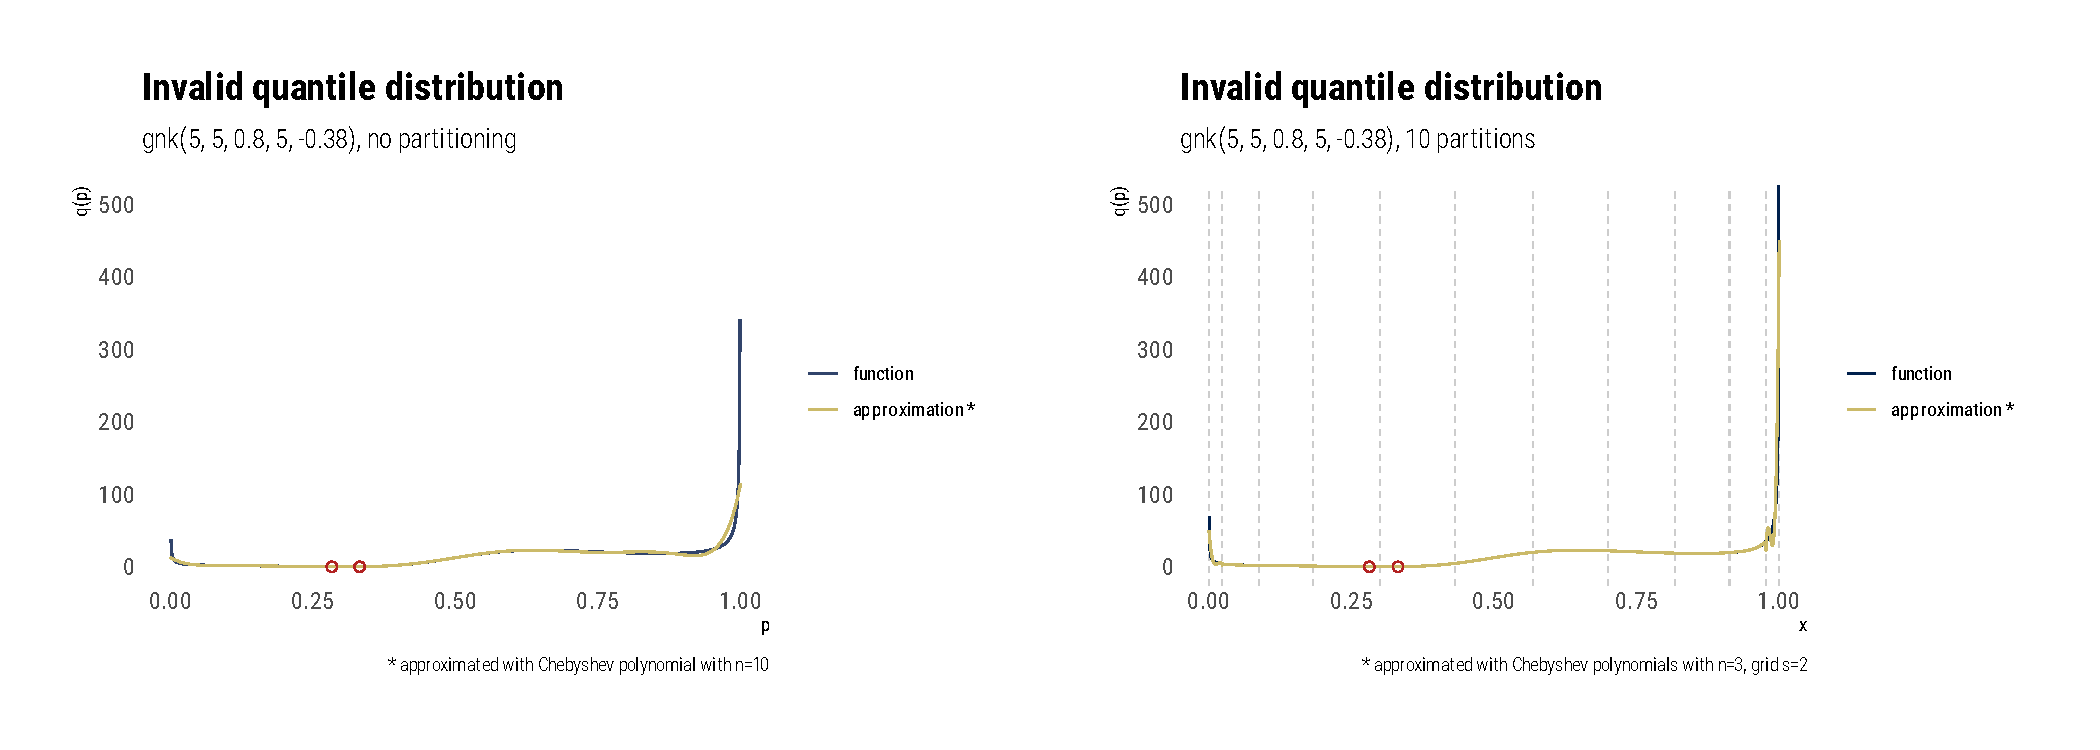
\includegraphics{ilbm_article_files/figure-latex/chebyshev-roots-gnk-graph-1} 

}

\caption{Chebyshev polynomial approximation: valid QDF and true-positive proxy roots}\label{fig:chebyshev-roots-gnk-graph}
\end{figure}

Figure \ref{fig:chebyshev-roots-gnk-graph} illustrates the ideas presented in this section. The \emph{g-and-k} distribution \(GnK(5,5,0.8,5,-0.38)\) has an invalid QF. Graph on the left shows an approximation of QDF with Chebyshev polynomials of degree 10 without partitioning the range. Two roots are identified and they are correctly highlighting the area where QDF takes negative values. The function range can also be partitioned as shown on the graph to the right. Here partitioning is performed using the S-shaped scheme implemented in \texttt{qpd::make\_pgrid()}. The parameter \texttt{s} is passed to the beta inverse transform so that the partitions are made at the points corresponding to \(Q_{beta}(\{u_{(M)} \}, s,s)\), where \(\{u_{(M)} \}\) is a uniformly distributed grid of \(M\) points. Uneven grid facilitates better fit in the tails of the QDF, but most importantly, allows us to use lower degree polynomials. In the partitioned case presented on the right, we used cubic Chebyshev polynomial fit on each of the 10 segments.

\begin{figure}

{\centering 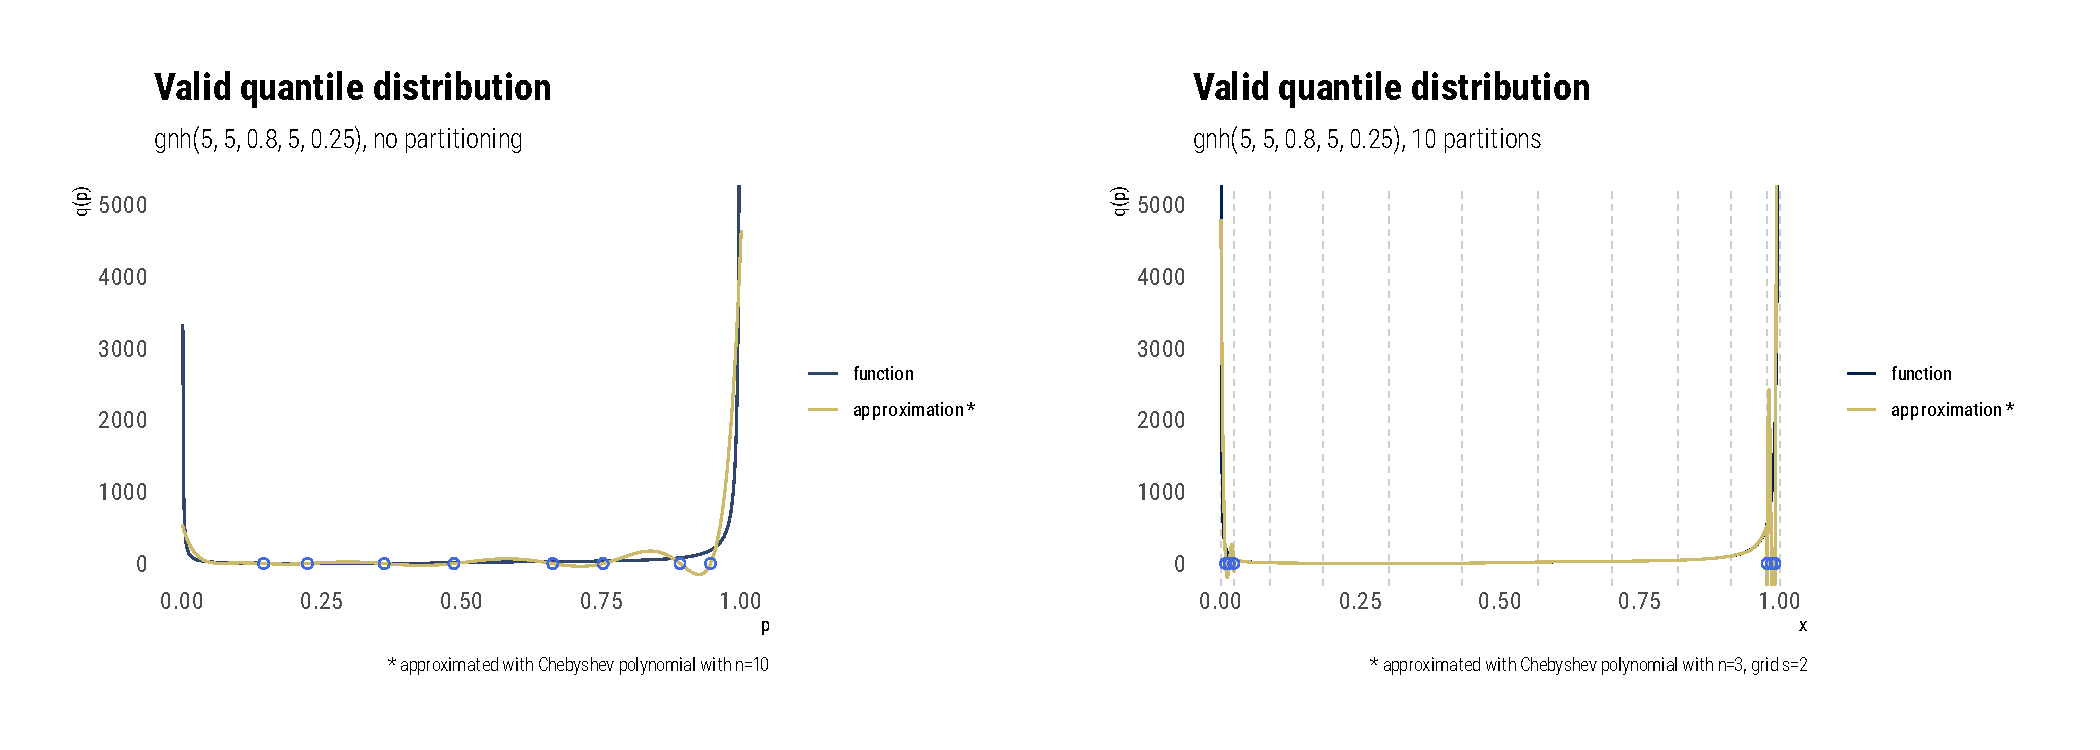
\includegraphics{ilbm_article_files/figure-latex/chebyshev-roots-gnh-graph-1} 

}

\caption{Chebyshev polynomial approximation: valid QDF and false-positive proxy roots}\label{fig:chebyshev-roots-gnh-graph}
\end{figure}

Unfortunately, not all quantile functions are behaving as nicely. Figure \ref{fig:chebyshev-roots-gnh-graph} presents a valid \emph{g-and-h} distribution which we also approximated with a Chebyshev polynomial of degree 10. All roots are false. They appear because of extreme curvature of the QDF in the tails. When the range is partitioned, the false roots move into the outermost bins, which are in fact ``safest'' areas of the QDF curve (above the y-axis) even by visual inspection. We need to evaluate the function less than 10 times to refute the roots and assure ourselves that the function is valid. Increasing the degree of the fitted polynomial (or increasing the number and/or density of the QDF range partitions) might reduce the number of false roots and move them even further out towards the tails. Given the low number of roots, and relatively inexpensive evaluation of QDF, these strategies may not be justifiable.

  \bibliography{ilbm-article.bib}

\end{document}
